\chapter{Implementación digital} \chapterlabel{Informe/7-ImplementacionDigital} \label{cap:Implementacion digital}

En este capítulo se realiza el diseño de un compensador y estimador en el dominio digital para ser implementados en un microcontrolador que se conecta de manera externa a la placa de control. Para el primero se sigue la misma estrategia que se utiliza en la etapa de compensación analógica, descripta en el capítulo \ref{cap:Compensador Analogico}, pero con las consideraciones necesarias para trabajar con sistemas discretos. Para el segundo, se diseña un algoritmo encargado de obtener el valor de la distancia de separación $Y_g$ a partir de los valores obtenidos al muestrear la tensión entregada por el sensor de efecto Hall.

Por otra parte, se diseñan los circuitos de interfaz encargados de muestrear, reconstruir y adaptar los niveles de tensión de las señales que interactúan entre la placa de control y el microcontrolador.


\section{Descripción general}

 La implementación digital consiste en realizar la estimación de posición y el control de la planta por medio de un microcontrolador. Se utiliza un kit de desarrollo basado en el microcontrolador STM32F072, que contiene un conversor digital analógico (DAC) y un conversor analógico digital (ADC), ambos de 12 bits y $3.3\:V$ de referencia. 

 En la figura \ref{fig:diag-en-bloques-digital} se muestra un diagrama en bloques general de la implementación digital del sistema. Es posible observar que se ingresa al microcontrolador a través de un canal del ADC, con una tensión de referencia ($V_{y_{ref}}$) proporcional a la distancia de separación deseada, que es la misma utilizada en la implementación analógica. Además, se ingresa por medio de otro canal del ADC con la tensión de salida del sensor de efecto hall ($V_{IL_{feed}}$). Por otro lado, mediante un DAC, se ingresa al controlador de corriente $G_{IL}(s)$, que actúa sobre la planta $G_P(s)$, y modifica la distancia de separación.

% Por medio de un ADC y el sensor de efecto Hall, se muestrea una tensión proporcional a la corriente que circula por el electroimán. Se implementa un algoritmo de estimación dentro del microcontrolador que permite obtener una posición estimada $Y(z)$. Este está representado por la transferencia $H(Z)$.


\begin{figure}[H]
	\centering
	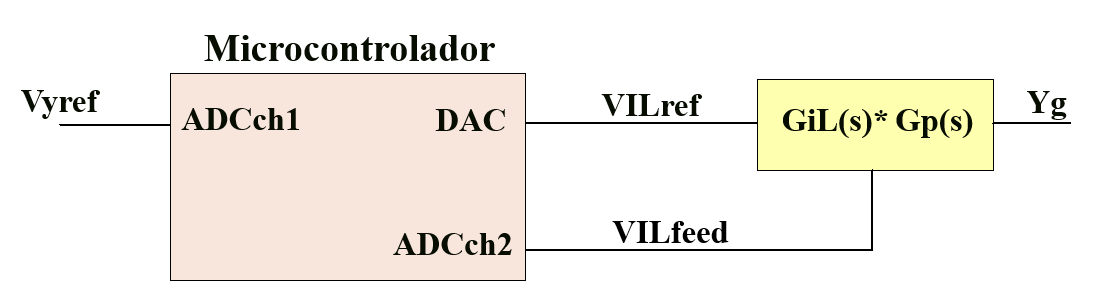
\includegraphics[scale=0.5]{Diagrama-en-bloques-digital2.png}
	\caption{Diagrama en bloques de la implementación digital.}
	\label{fig:diag-en-bloques-digital}
\end{figure}

%\colorbox{blue}{yo dejaría el de arriba que representa mejor que la entrada al sistema digital es la corriente. pero el de abajo nos sirve para el diseño del compensador también}
%
%Abstrayéndose de la matemática que se realiza dentro del microcontrolador para la estimación de posición, se puede simplificar el diagrama al que se muestra en la figura \ref{fig:diag-en-bloques-digital-simplif}, en la que:

%\begin{equation} 
%	G_T(s) = G_P(s) * G_{iL}(s).
%\end{equation}

%\begin{figure}[H]
%	\centering
%	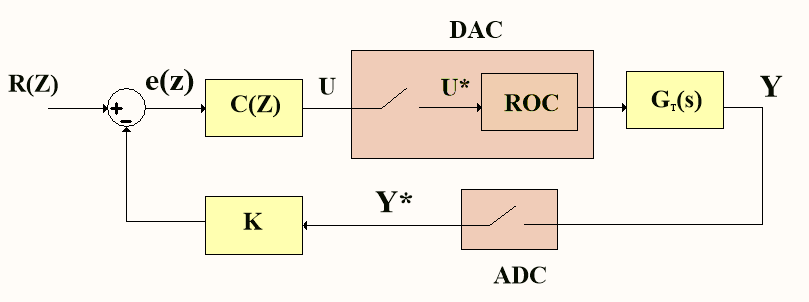
\includegraphics[scale=0.5]{Diagrama-en-bloques-digital-simplificado.png}
%	\caption{Diagrama en bloques de la etapa digital simplificado.}
%	\label{fig:diag-en-bloques-digital-simplif}
%\end{figure}
%
%\colorbox{blue}{acá arrancaría con una sección general que sea algoritmo de estimación y dentro de ella iría lo de frecuencia de muestreo, etc...}

% En la figura \ref{fig:diag-en-bloques-digital} se muestra un diagrama en bloques general de la implementación digital del sistema. Todos los bloques dentro del microcontrolador están representados por funciones transferencia en el dominio de la variable Z. \colorbox{red}{creo que sería medio complicado explicar qué es z}. Es posible observar que se ingresa al microcontrolador a través de un ADC, con una tensión de referencia ($V_{y_{ref}}$) proporcional a la distancia de separación deseada, que es la misma utilizada en la implementación analógica. Esta es multiplicada por la ganancia de entrada $G_{in}$ y luego es comparada con la posición estimada $Y(z)$. El resultado $e(z)$ es la entrada del compensador digital $C(z)$. Por medio de un DAC, la salida del compensador digital ingresa al controlador de corriente $G_{IL}(s)$, que actúa sobre la planta $G_P(s)$, y modifica la distancia de separación.
%
%Por medio de un ADC y el sensor de efecto Hall, se muestrea una tensión proporcional a la corriente que circula por el electroimán. Se implementa un algoritmo de estimación dentro del microcontrolador que permite obtener una posición estimada $Y(z)$. Este está representado por la transferencia $H(Z)$.
%
%\colorbox{blue}{yo dejaría el de arriba que representa mejor que la entrada al sistema digital es la corriente. pero el de abajo nos sirve para el diseño del compensador también}
% Abstrayéndose de la matemática que se realiza dentro del microcontrolador para la estimación de posición, se puede simplificar el diagrama al que se muestra en la figura \ref{fig:diag-en-bloques-digital-simplif}, en la que:
%
%\begin{equation} 
%	G_T(s) = G_P(s) * G_{iL}(s).
%\end{equation}
%
%\begin{figure}[H]
%	\centering
%	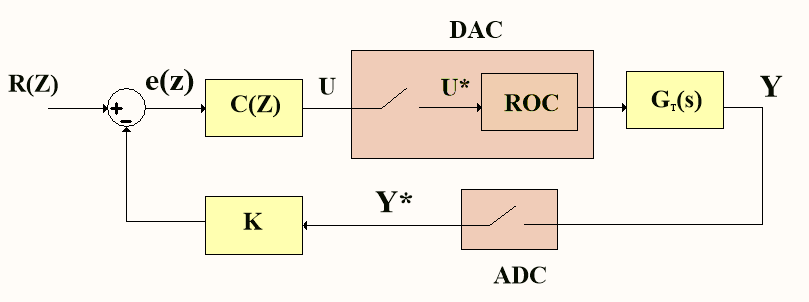
\includegraphics[scale=0.5]{Diagrama-en-bloques-digital-simplificado.png}
%	\caption{Diagrama en bloques de la etapa digital simplificado.}
%	\label{fig:diag-en-bloques-digital-simplif}
%\end{figure}
%
%\colorbox{blue}{acá arrancaría con una sección general que sea algoritmo de estimación y dentro de ella iría lo de frecuencia de muestreo, etc...}


\section{Consideraciones para el dominio discreto}\label{consideraciones_sistemas_discretos}

Como se mencionó previamente, para la implementación digital se van a tomar muestras de la señales de la planta y se las van a utilizar para implementar un algoritmo de compensación dentro del microcontrolador. 

Se desea implementar un compensador en el dominio discreto y controlar una planta continua. Para ello, es necesario convertir señales analógicas a discretas para poder utilizarlas en el algoritmo de control y viceversa para actuar sobre la planta. Para esto se utilizan conversores analógico digitales ($ADC$) y conversores digital analógicos ($DAC$). En la figura \ref{fig:diag-general-digital} se muestra un diagrama en bloques de un sistema de control con un compensador digital D(z) que controla una planta continua $G(s)$ cuya salida es la señal $C(s)$ y que es la variable que se desea controlar.

\begin{figure}[H]
	\centering
	\tikzset{%
	buffer/.style={
		draw,
		shape border rotate=270,
		regular polygon,
		regular polygon sides=3,
		fill=blue!20,
		node distance=2cm,
		minimum height=4em
	}
}

\tikzstyle{block} = [draw, fill=blue!20, rectangle, 
minimum height=2.5em, minimum width=3em]

%Acá se define eñ diagrama en bloques completo
\begin{tikzpicture}[auto, node distance=1cm,>=latex']
	% We start by placing the blocks
	\node [input, name=input] {R(z)};
	\node [sum, right of=input, node distance=1.5cm] (suma_externa) {+};
	\node [block, right=of suma_externa] (compensador) {$D(z)$};
	\node[block, right=of compensador] (dac) {DAC};
	%\node [block, right=of interno] (gil) {$G_{IL}(w)$};
	\node [block, right=of dac] (planta) {$G(s)$};
	\node [block, below=of dac] (realimentacion) {ADC};
	
	\node [output, right of=planta, node distance=3cm] (output) {};

%	% Once the nodes are placed, connecting them is easy. 
	\draw [draw,->] (input) -- node[pos=0.2]{$R(z)$} node[pos=0.9]{$+$}(suma_externa);
	\draw [draw,->] (suma_externa) -- node{$E(z)$} (compensador);
	\draw [draw,->] (compensador) -- node{$U(z)$} (dac);
	\draw [draw,->] (dac) -- node{$U(s)$} (planta);
	%\draw [draw,->] (gil) -- (planta);
	\draw [draw,->] (planta) -- node[name=y]{$C(s)$} (output);
%	\draw [draw,->] (amplificador) -- node[name=y]{$V_{deriv}$} (output);
	\draw [-] (y) |- (realimentacion);
	\draw [->] (realimentacion) -| node[pos=0.25]{$C(z)$} node[pos=0.99]{$-$} (suma_externa);
\end{tikzpicture}
	\caption{Diagrama en bloques de controlador digital.}	\label{fig:diag-general-digital}
\end{figure}

\colorbox{red}{¿Habría que agregar un ADC en la entrada con Vyref antes de R(z)?} yo creo que no haría falta porque este es un diagrama genérico que estaba en la pag de teoria de control, no es una representación de nuestro sistema. La entrada puede ser ya una señal digital


\colorbox{red}{¿Que sería C(s)?} una señal de salida, aparecía así en el diagrama de teoría de control



Para hacer la conversión entre el dominio digital al analógico, el DAC mantiene el valor entre cada muestra, actualizando el valor de la señal en cada intervalo de tiempo discreto ($T_s$). Este efecto se lo conoce como retenedor de orden cero ($ROC$) y se lo puede modelar con la ecuación \ref{eq_retenedor_orden-0}. Es importante tener en cuenta el efecto que agrega el $ROC$ sobre la planta al momento de diseñar el compensador, ya que puede afectar la estabilidad del sistema.

\begin{equation}\label{eq_retenedor_orden-0}
	ROC(s)=\frac{1-e^{-s*T_s}}{s}
\end{equation}

Para diseñar un compensador digital es necesario obtener una representación discreta de la planta que se quiere controlar, agregando la dinámica del ROC. Esta se puede obtener a través de la transformada Z por el método de invarianza al impulso:

\begin{equation*}
	G(z)= Z[ROC(s)*G(s)]
\end{equation*}

Una vez obtenido el modelo discreto de la planta con el efecto del ROC, se propone diseñar el compensador digital mediante el uso técnicas de diseño de compensadores analógicos. Para ello se hace uso de la transformada bilineal para convertir la transferencia en el dominio de Z, a una nueva variable W que es del tipo analógico. Esta se aplica sobre la representación discreta de la planta por medio de la siguiente expresión:


\begin{equation*}
	z=\frac{1+\frac{wT_s}{2}}{1-\frac{wT_s}{2}}
\end{equation*}



Una vez diseñado el compensador en el dominio analógico, se aplica la transformada bilineal inversa y se obtiene su equivalente en el plano transformado Z para ser implementado en el microcontrolador. Este compensador $D(z)$ es luego convertido, por medio de la transformada Z inversa, a una ecuación en diferencias que relaciona la salida $u[n]$ con la entrada $e[n]$. 


\colorbox{red}{Releer y ver si quedó bien}

%\subsection{Transferencias de la planta y del controlador de corriente}
%
%Para el análisis del compensador digital se parte de las transferencias de la planta $G_P(s)$ y del controlador de corriente $G_{iL}(s)\ $ en dominio analógico para una masa de $30 \:kg$.
%
%\begin{equation} 
%	\begin{aligned}
%		G_T(s)[M=30kg]&=G_P(s)*G_{iL}(s)&=\frac{-87.7}{\ (s-70)\ (s+70)\ (s+12.17)}\\
%	\end{aligned}
%\end{equation}
%
%Para incluir el efecto del ROC a esta transferencia se aplica la transformada z por el método de invarianza al impulso. 
%
%\begin{equation*}
%	G_T(z)=Z\{\frac{(1-e^{-s*T_s})}{s}*G_T(s)\}=(1-z^{-1})*Z\{\frac{G_T(s)}{s}\})
%\end{equation*}
%
%Para obtener esta transformada es necesario conocer el período de muestreo $T_s=\frac{1}{F_s}$. A continuación se hará un análisis de cual será el algoritmo de control y se escoge una $F_s$ para luego obtener la transferencia del controlador $G_c(z)$.



\section{Diseño del algoritmo de estimación}

En esta sección se diseña el algoritmo que realiza la estimación de distancia de entrehierro $Y_g$ a partir de las muestras tomadas por el ADC de la tensión de salida del sensor de efecto Hall.

La señal que entra al ADC es la salida del sensor de efecto Hall $V_{IL_{feed}}$, que está dada por:

\begin{equation*}
	V_{IL_{feed}}=K_h*I_L+0.1\:V
\end{equation*}

Donde $K_h$ es la ganancia del sensor de efecto Hall. Como la señal $V_{IL_{feed}}$ tiene un punto de operación de $0.1\:V$, se decide realizar el análisis adoptando una nueva señal $V_h$ tal que:

\begin{equation*}
	V_h=V_{IL_{feed}}-0.1\:V=K_h*I_L
\end{equation*}


La conversión entre la señal $V_{IL_{feed}}$ y $V_h$ será realizada dentro del microcontrolador luego de muestrear la señal de entrada con ADC.

La estimación de distancia de entrehierro se obtendrá al medir la pendiente de la señal $V_h$. Dentro del microcontrolador se implementa un algoritmo para procesar las muestras y calcular la distancia estimada. 

\subsection{Determinación de la frecuencia de muestreo}

El ADC toma muestras de la señal en su entrada de manera periódica. Es importante realizar un análisis de cuál es la frecuencia con la que debe tomarlas, de manera de obtener una señal adecuada para realizar la estimación.

Como se vio en el capitulo \ref{cap:ControladorCorriente}, la forma de onda de la salida del sensor de efecto Hall es triangular y presenta una frecuencia de conmutación ($F_{planta}$) que varía en función de la distancia de entrehierro. Se puede calcular como:

\begin{equation} \label{eq_frecuencia-de-muestreo}
	F_{planta}(Y_g)=\frac{V_{cc}}{2 * L(Y_g) * \Delta I_L}
\end{equation}


Al aplicar en la ecuación \ref{eq_frecuencia-de-muestreo} los valores de inductancia ($L\:[mHy]$) obtenidos en las mediciones realizadas sobre el electroimán (ver tabla \ref{tab_mediciones_inductancia}), se calcula la frecuencia de conmutación  $(F_{planta}\:[Hz])$. Los resultados se muestran en la tabla \ref{frecuencias-calculadas}.



\begin{table}[H]
	\begin{center}
		\begin{tabular}{| c | c | c |}
			\hline
			$Y_g\:[mm]$ & $L\:[mHy]$ & $F_{planta}\:[Hz]$\\ \hline
			2 & 22.64 & 1060\\ \hline
			3 & 18.8 & 1276\\ \hline
			4 & 16.44 & 1459\\ \hline
			5 & 14.9 & 1632\\ \hline
		\end{tabular}
		\caption{Valores de frecuencia calculados a partir de las mediciones de inductancia realizadas.}
		\label{frecuencias-calculadas}
	\end{center}
\end{table}


 Para la estimación de distancia de entrehierro es necesario medir la pendiente de la onda triangular sin alterar demasiado su forma. Debido a que la conversión realizada por el ADC recorta el contenido de frecuencia de la señal a partir de la mitad de frecuencia de muestreo, se debe elegir esta última de manera que se conserve la información de la pendiente.  Por lo tanto, para reconstruirla correctamente se decide que la frecuencia de muestreo del ADC sea al menos el doble de la frecuencia de la 5° armónica para el caso de distancia de entrehierro en que $F_{planta}$ es la mayor. Para tener cierto margen, se adopta que la frecuencia de muestreo sea 2.5 veces superior. Es decir:

\begin{equation} 
	F_{ADC} \geq 2.5 * 5 * F_{planta_{max}} \Rightarrow  F_{ADC} \geq 2.5 * 5 * 1632\:Hz \Rightarrow F_{ADC} \geq 20400\:Hz
\end{equation}


 De esta forma, se adopta una frecuencia de muestreo para el ADC de  $25\:kHz$. Con este valor es posible obtener 15 muestras en un período de la triangular para el caso de $F_{planta}$ máxima. Como la señal crece o decrece durante medio ciclo, se pueden tomar 7 muestras para identificar la pendiente. En el caso de que la señal presente la $F_{planta}$ mínima, se pueden tomar 23 muestras en un ciclo. Esto se traduce en 11 muestras para la pendiente de subida o bajada. 


\subsection{Adquisición y procesamiento de las muestras} \label{sec_adquisicion_y_procesamiento}

En esta sección se desarrolla el algoritmo ideado para estimar la distancia de entrehierro. Este se puede observar en el diagrama de flujo \ref{fig:procesamiento-muestras-adquiridas}.


\begin{figure}[H]
	\centering
	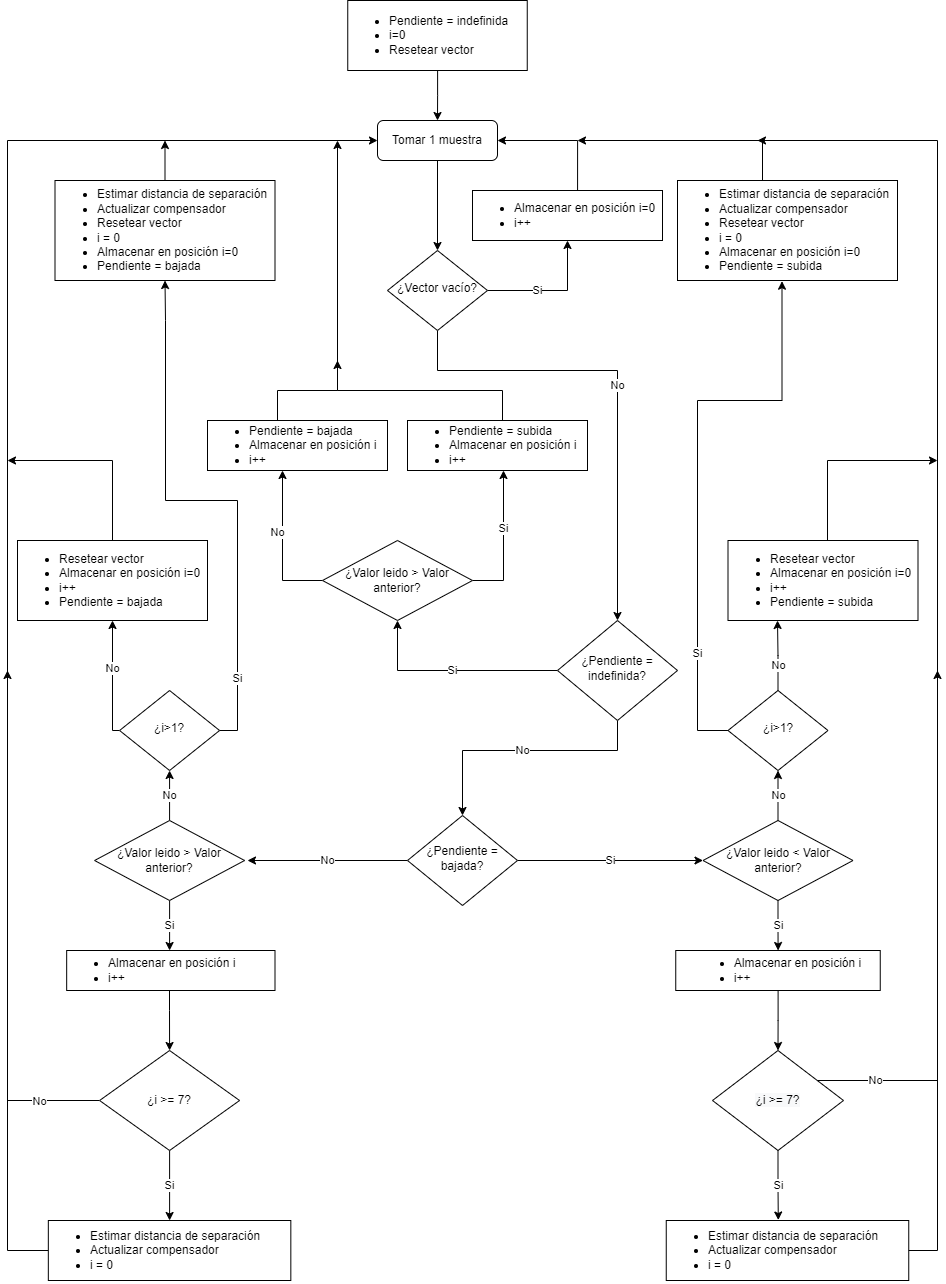
\includegraphics[scale=0.5]{Estimación de posición-Página-2.drawio.png}
	\caption{ Diagrama de flujo del procesamiento de las muestras adquiridas.}
	\label{fig:procesamiento-muestras-adquiridas}
\end{figure}

%Cada muestra de tensión tomada de la señal $V_h$ se almacena en un vector de 7 posiciones. Se elige este tamaño considerando el caso extremo de frecuencia, en el que solo se pueden obtener 7 muestras por semiciclo. Para poder discernir entre pendientes de bajada y de subida, se verifica en cada muestra si el valor leído es mayor o menor al almacenado en la posición anterior. En caso de que sea mayor al anterior, significa que se está muestreando la pendiente positiva de la onda triangular. La distinción entre pendientes positivas y negativas es importante puesto que permite aplicar la compensación de la resistencia interna al igual que se realiza en el estimador analógico. 
%
%Cada vez que el vector se completa, se realiza el cálculo de la derivada con el valor máximo y mínimo almacenado. Con este resultado, se hace la estimación de la posición y se actualiza la entrada al compensador digital.
%
%En caso de haber completado las 7 posiciones del vector y la pendiente persiste con el mismo signo, el vector comienza a llenarse nuevamente desde la posición inicial, sobrescribiendo los valores mas antiguos. Por lo tanto, pueden ocurrir dos situaciones. La primera es que se detecte un cambio de pendiente antes de completar nuevamente el vector, con lo cual se calcula la derivada con los valores extremos almacenados teniendo en cuenta el tiempo transcurrido ($K$ períodos de muestreo), y se actualiza la entrada al compensador. La segunda, es que se vuelva a completar el vector, en cuyo caso también se hace la actualización. La diferencia entre estas dos situaciones es el tiempo transcurrido hasta que se obtiene una nueva estimación. En este último, se hace cada 7 períodos de muestreo mientras que en el primero se realiza en ``$n-1$'' períodos luego de la última actualización, siendo “n” la cantidad de muestras que se almacenaron en el vector incompleto ($n>1$).
%
%Luego de detectar un cambio de pendiente, el
%proceso vuelve a iniciar con el vector vacío.
%
%Al utilizar este método de estimación, puede ocurrir que se obtenga una nueva estimación en 7 periodos de muestreo del ADC, o incluso en menos. Por lo tanto se tiene un estimador de distancia de entrehierro con frecuencia de actualización variable. Esto será importante luego al momento de diseñar el compensador digital. Para hacerlo, se debe considerar el caso en que la frecuencia de actualización es la menor. Por lo tanto el compensador digital se debe diseñar con una frecuencia de muestreo de $F_S=25/7 \:kHz = 3.5\:kHz$.

Cada muestra de tensión tomada de la señal $V_h$ se almacena en un vector de 7 posiciones. Para poder discernir entre pendientes de bajada y de subida, se verifica en cada muestra si el valor leído es mayor o menor al almacenado en la posición anterior. En caso de que sea mayor al anterior, significa que se está muestreando la pendiente positiva de la onda triangular. La distinción entre pendientes positivas y negativas es importante puesto que permite aplicar la compensación de la resistencia interna al igual que se realiza en el estimador analógico. 

Cada vez que el vector se completa, se realiza el cálculo de la derivada con el valor máximo y mínimo almacenado. Con este resultado, se hace la estimación de la posición y se actualiza la entrada al compensador digital.

En caso de haber completado las 7 posiciones del vector y la pendiente persiste con el mismo signo, el vector comienza a llenarse nuevamente desde la posición inicial, sobrescribiendo los valores mas antiguos. Por lo tanto, pueden ocurrir dos situaciones. La primera es que se vuelva a completar el vector y la segunda es que se detecte un cambio de pendiente antes de completarlo. En ambos casos, el cálculo de la estimación se realiza con los valores extremos almacenados. Sin embargo, la diferencia radica en el tiempo transcurrido entre actualizaciones del compensador. En el primero se realiza cada 7 períodos de muestreo ($7*T_s$) mientras que en el segundo cada K períodos ($K*T_s$), donde “$K=n-1$” y $n$ representa la cantidad de muestras que se almacenaron en el vector incompleto ($n>1$).

Luego de detectar un cambio de pendiente, el proceso vuelve a iniciar con el vector vacío. En caso de que se detecte un cambio de pendiente antes de completar por primera vez el vector, el calculo de la estimación se realiza con los valores extremos almacenados teniendo en cuenta el tiempo trascurrido ($K*T_s$), con $n>1$. En este caso, el tiempo de actualización del compensador también es de ($K*T_s$).

Al utilizar este método de estimación, puede ocurrir que se obtenga una nueva estimación en 7 periodos de muestreo del ADC, o incluso en menos. Por lo tanto se tiene un estimador de distancia de entrehierro con frecuencia de actualización variable. Esto será importante luego al momento de diseñar el compensador digital. Para hacerlo, se debe considerar el caso en que la frecuencia de actualización es la menor. Por lo tanto el compensador digital se debe diseñar con una frecuencia de muestreo de $F_S=(25\:kHz)/7 = 3.5\:kHz$.






%La derivada se calcula con todos los valores disponbles en el vector. No importa si es la segunda vez que se esta completando el vector..
%El compensador se actualiza cada vez que se obtiene una nueva estimación. Por lo tanto, puede ser cada 7 períodos o menos (buffer incompleto).


\subsection{Estimación digital de la posición}

En el capitulo \ref{cap:Estimador Analogico} se analizó la relación entre la distancia del entrehierro con la pendiente de la corriente en el electroimán. Se llegó a la expresión \ref{eq_Yg_despejada}, que se repite a continuación:

\begin{equation} \label{eq_yg_vs_derivada}
	Y_g = 5.136*10^{-6}*|\frac{di_L}{dt}|- 3.472*10^{-3} [m]
\end{equation}

A partir de la expresión \ref{eq_yg_vs_derivada} se puede obtener la distancia de entrehierro midiendo la pendiente de la corriente. Sin embargo, esta expresión fue calculada suponiendo que no se generaba una caída de tensión en la resistencia interna del electroimán ($R_L$), obteniendo una pendiente teórica. Esta caída provoca que la tensión efectiva aplicada sobre la inductancia sea distinta para el semiciclo de subida que para el de bajada. De esta forma, la onda triangular presenta diferentes pendientes (en valor absoluto) para cada caso. Esta se representa como $(\frac{di_L}{dt})_{Real}$ y es la que se mide al utilizar el ADC. La relación entre esta y la teórica se da por:

\begin{equation} \label{eq_derivada_real}
	(\frac{di_L}{dt})_{Real}=(\frac{di_L}{dt})_{Teorica}-\frac{R_L*I_L}{L(Y_g)}
\end{equation}

Por lo tanto al despejar la derivada teórica de la expresión \ref{eq_derivada_real} se obtiene:

\begin{equation} \label{eq_derivada_teorica}
	(\frac{di_L}{dt})_{Teorica}=(\frac{di_L}{dt})_{Real}+\frac{R_L*I_L}{L(Y_g)}
\end{equation}


Para calcular la derivada real de la pendiente dentro del microcontrolador se aproxima como la resta entre la muestra de corriente en un instante ($I_L[n]$) menos la muestra mas antigua en el vector ($I_L[n-K]$) sobre el intervalo de tiempo transcurrido entre ellas ($K*T_S=\frac{K}{F_S}$). Al considerar este cálculo de la derivada y utilizar \ref{eq_derivada_teorica} en \ref{eq_yg_vs_derivada}, se obtiene:

\begin{equation} \label{eq_yg_vs_IL}
	Y_g[n] = 5.136*10^{-6}* |\frac{I_L[n]-I_L[n-K]}{K*T_S}+\frac{R_L*I_L[n]}{L(Y_g)[n-1]}| - 3.472*10^{-3} [m]
\end{equation}

$V_h$ es la tensión proporcional a la corriente que circula por el electroimán multiplicada por la ganancia $K_h=53.3\:mV/A$. Esta señal se puede separar en dos componentes: $\hat{V_h}$  correspondiente a la componente alterna de tensión y $\bar{V_h}$ a la continua:


\begin{equation} 
	V_h[n] = \bar{V_h}[n] + \hat{V_h}[n] = K_h * (\bar{I_L}[n] + \hat{I_L}[n])
\end{equation}

 Para la estimación de la posición se utiliza el término de alterna mientras que para compensar el error introducido por la resistencia interna del electroimán se utiliza el de continua. Por lo tanto reemplazando $I_L=\frac{V_h}{K_h}$ en la ecuación \ref{eq_yg_vs_IL}, se obtiene:

\begin{equation}
	\resizebox{.8\hsize}{!}
	{
	$Y_g[n] = 5.136*10^{-6}*|\frac{\hat{V_h}[n]-\hat{V_h}[n-K]}{K*K_h*T_S} + \frac{R_L*\bar{V_h}[n]}{K_h*L(Y_g)[n-1]}|-3.472*10^{-3}[m]$
	}
\end{equation}

El término $\bar{V_h}[n]$ se obtiene de sensar el valor medio de la tensión $V_h$ mediante un canal del ADC.

Por otro lado, el valor de $L(Y_g)[n-1]$ se obtiene al aplicar el valor estimado de posición anterior en la ecuación \ref{eq_inductancia}. El cálculo de esta expresión se obtuvo a partir de la linealización de la inductancia en función de las mediciones realizadas sobre el electroimán.


\begin{equation} \label{eq_inductancia}
	L(Y_g)[n] = -2.56*Y_g[n]+0.0271\:Hy
\end{equation}

 Por lo tanto, la ecuación correspondiente en el tiempo discreto resulta:

\begin{equation}
	\resizebox{.8\hsize}{!}
	{
	$Y_g[n] = 5.136*10^{-6}*|\frac{\hat{V_h}[n]-\hat{V_h}[n-K]}{K*K_h*T_S} + \frac{R_L*\bar{V_h}[n]}{K_h*(2.56*Y_g[n-1]+0.0271)}|-3.472*10^{-3}\:[m]$
	}
\end{equation}

\begin{equation}
	\resizebox{.8\hsize}{!}
	{
	$
	Y_g[n] = 96.3*10^{-6}*|\frac{\hat{V_h}[n]-\hat{V_h}[n-K]}{K*T_S} + \frac{R_L*\bar{V_h}[n]}{(2.56*Y_g[n-1]+0.0271)}|-3.472*10^{-3}\:[m]
	$
	}
\end{equation}


Donde $V_h[n]$ se refiere a la muestra más reciente en el vector y $V_h[n-K]$ a la más antigua.

Es importante notar que los coeficientes del estimador deben calcularse justo antes de realizar una nueva estimación,  en función de la cantidad de muestras que se utilizan para el cálculo de la pendiente. Si bien el estimador presenta una frecuencia de actualización variable, los coeficientes del compensador digital no se ven modificados ya que se calculan teniendo en cuenta la frecuencia de actualización más lenta.


\subsection{Resolución en posición}

En esta sección se analiza cuál es la resolución en posición que se puede obtener con el algoritmo de estimación diseñado.

Una variación de posición ($\Delta Y_g$) produce un cambio de inductancia ($\Delta L(Y_g)$) que se traduce en un cambio de frecuencia ($\Delta F_{planta}$). Para poder detectar el mínimo cambio de posición en un período de muestreo se debe tener una resolución tal que permita discernir ese cambio de frecuencia.


A partir de la expresión linealizada de la inductancia \ref{eq_induct_practica} y la ecuación \ref{eq_frecuencia-de-muestreo} es posible obtener el valor de frecuencia para una separación de $Y_g=2.1\:mm$. Esta resulta en $F_{planta}[2.1\:mm] = 1104.8\:Hz$. De esta forma, al conocer el valor de frecuencia para $2\:mm$, el cual es de $F_{planta}[2\:mm] = 1060\:Hz$, es posible obtener la variación de frecuencia para un ($\Delta Y_g$) mínimo de  $0.1\:mm$. Este valor puede obtenerse como:

\begin{equation} 
	\Delta F_{planta} = F_{planta}[2.1\:mm] - F_{planta}[2\:mm] = 44.8\:Hz
\end{equation}

 Las pendientes para el peor caso se da con la menor variación de tensión entre muestras. Es decir, para el caso de en que $F_{planta}$ es la mínima. En la ecuación \ref{eq_pendiente} se muestra el cálculo de la pendiente de la onda triangular en función de la frecuencia de conmutación.

\begin{equation} \label{eq_pendiente}
	P(F_{planta}) = \frac{\Delta V}{T_{planta}/2} = 2*K_h*\Delta i_L*F_{planta} = 2 * 0.0533 * 0.5 * F_{planta}
\end{equation}

 A partir de la ecuación \ref{eq_pendiente} es posible obtener el valor de la pendiente para la mínima frecuencia de conmutación y la de su incremento correspondiente a una variación en la posición de $0.1\:mm$. Esta situación se representa en la figura \ref{fig:variacion-de-pendiente}.

\begin{equation} 
	\begin{aligned}
		&P(F_{planta_{min}}) = 56.49\:[V/s] \\
		&P(F_{planta_{min}} + \Delta F_{planta}) = 58.89\:[V/s] \\
	\end{aligned}
\end{equation}

\begin{figure}[H]
	\centering
	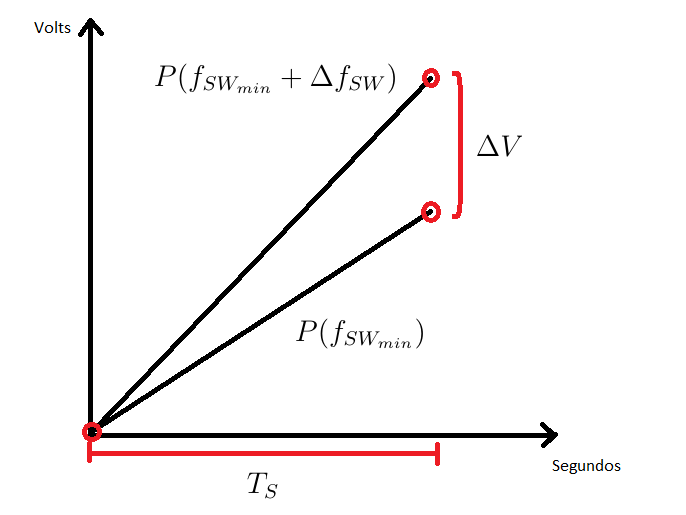
\includegraphics[scale=0.5]{Variacion-de-pendientes.png}
	\caption{Variación de pendiente ante mínimo cambio de posición.}
	\label{fig:variacion-de-pendiente}
\end{figure}

\colorbox{red}{en el texto antes deciamos Fplanta y fsw como que eran lo mismo. cambié todas por Fplanta pero en la imagen quedó com fsw... que hacemos?}

 Por lo tanto, para poder diferenciar las pendientes, la resolución del ADC debe ser menor o igual a $\Delta V$.

\begin{equation} 
	\begin{aligned}
		V1 &= P(F_{planta_{min}} + \Delta F_{planta})* T_{ADC} \\
		V2 &= P(F_{planta_{min}})* T_{ADC} \\		 
	\end{aligned}
\end{equation}

 Al considerar $F_{ADC} = 25\:kHz$:

\begin{equation} 
	\Delta V_{ADC} = T_S * [P(F_{planta_{min}} + \Delta F_{planta}) - P(F_{planta_{min}})] = 96\:\mu V
\end{equation}



 Este resultado indica que se necesita una resolución en el ADC de $96\:\mu V$. Este valor depende de la cantidad de bits (N) que utiliza el ADC y de su tensión de referencia ($V_{ref}$), de manera que:
 
 \begin{equation*}
 	\Delta V_{ADC}=\frac{V_{ref}}{2^N}
 \end{equation*}

Al usar un ADC de 12 bits, se necesitaría una tensión de referencia $V_{ref} = 0.39\:V$ para lograr la resolución de $96\:\mu V$. Sin embargo, este valor resulta demasiado bajo y no sirve si se quiere medir la tensión de salida del sensor de efecto Hall de manera directa. Por lo tanto, se decide diseñar un circuito que permita realizar la estimación manteniendo la tensión de referencia en $3.3\:V$ y teniendo una resolución $\Delta V_{ADC}=0.8\:mV$.

\subsection{Adaptación de señal de entrada al ADC}\label{sec_adaptacion_señal_vh_ADC}

En esta sección se analiza una estrategia para poder medir la señal $V_h$ con la precisión deseada.

La corriente que circula por el electroimán presenta una componente de continua y otra de alterna. La primera excursiona entre $0\:A$ y $30\:A$ mientras que la segunda varía entre $\pm 250\:mA$ en torno al valor medio, con forma de onda triangular. Esto significa que la señal $V_h$ está compuesta por un valor medio que varía entre $0\:V$ y $1.6\:V$, y un valor de alterna de $26.7\:mV_{pp}$.

Se propone realizar una adquisición separada de ambas componentes de la tensión $V_h$. De esta manera se puede ingresar a un canal del ADC con $\bar{V_h}$ y en otro canal ingresar con $\hat{V_h}$. Esto permite amplificar la señal $\hat{V_h}$ para lograr la resolución deseada. Además se agrega un punto de operación de $2.5\:V$ a esta señal amplificada.

Debido a que el ADC permite una excursión entre $0\:V$ y $3.3\:V$, la máxima ganancia posible es de 60 veces para la componente de alterna.

\begin{equation*}
	3.3 \:V = \frac{26.7\:mV_{pp}}{2}*G_{max}+2.5\:V
\end{equation*}


Por otro lado, para medir con la resolución en posición deseada de $0.1\:mm$ se la debe amplificar 9 veces como mínimo.

\begin{equation*}
	0.8\:mV_{pp} = 96\:\mu V * 9
\end{equation*}

Por lo tanto, se adopta una ganancia de 50, y se obtiene una excursión máxima de $3.17\:V$ (es decir, $0.67\:V$ sobre el punto de operación).

Para realizar la separación de las componentes de la señal $V_h$ se utiliza un circuito con una ganancia de 50, un punto de operación de $2.5\:V$ en la salida, una frecuencia de corte inferior de $100\:Hz$ para bloquear el valor medio y una frecuencia de corte superior de $12.5\:kHz$ correspondiente a la mitad de la frecuencia de muestreo del ADC. De esta forma, se evita el solapamiento de la señal muestreada.

%La frecuencia de  corte superior de $12.5\:kHz$ corresponde a la de un filtro anti-solapamiento. El uso de estos filtros antes de la discretización de los datos es necesario ya que al hacerlo aparece una réplica espectral de la señal muestreada desplazada a la frecuencia de muestreo y a sus n-múltiplos. Esta réplica puede mezclarse con la señal deseada. 
%\begin{itemize}
%	\item Ganancia: 50
%	\item \textsl{set-point} de $2.5\:V$
%	\item Frecuencia de corte inferior: $100\:Hz$
%	\item Frecuencia de corte superior: $12.5\:kHz$
%\end{itemize}



Al considerar la ganancia elegida,  la pendiente de la onda triangular resulta:

\begin{equation} 
	P(F_{planta}) = 50 * [0.0533 * 0.5 * (F_{planta}*2)]\:[\frac{V}{s}]
\end{equation}

 Al reemplazar para el incremento de frecuencia se obtiene: 

\begin{equation*} 
	\begin{aligned}
		&P(F_{planta_{min}}) = 2824.9 \: [\frac{V}{s}]\\
		&P(F_{planta_{min}} + \Delta F_{planta}) = 2944.29 \: [\frac{V}{s}]\\		 
	\end{aligned}
\end{equation*}

 Por lo tanto, resulta:


\begin{equation*} 
	\resizebox{.9\hsize}{!}
	{
	$\Delta V_{ADC} = T_S * [P(F_{planta_{min}} + \Delta F_{planta}) - P(F_{planta_{min}})] = 0.1177\:V - 0.1129\:V = 4.7\:mV$
	}
\end{equation*}


 De esta manera, como la resolución del ADC es de $0.8\:mV$, resulta suficiente para identificar el mínimo cambio de pendiente.


\section{Circuitos de acondicionamiento de señales para el microcontrolador}
En esta sección se realiza el diseño circuital de las etapas de acondicionamiento correspondientes a las señales que interactúan entre el microcontrolador y el sistema analógico. Se implementan protecciones de sobre tensión en las entradas del microcontrolador, filtros anti-solapamiento y de reconstrucción de señales y ganancias para adecuar niveles de tensión.

\subsection{Circuitos de acondicionamiento de señales para el ADC}

 Para convertir los valores analógicos de las señales de referencia de posición y salida del sensor de efecto Hall, se utiliza el ADC del microcontrolador con una tensión de referencia de $3.3\:V$ y una frecuencia de muestreo de $25\:kHz$. Se agrega circuitería de filtrado, ganancia y protección en las entradas del ADC para hacerlas aptas para ingresar al microcontrolador.
 
\subsubsection{Referencia de posición} \label{sec_referencia_pos}

 Para indicar al microcontrolador la distancia de separación deseada se utiliza la señal  $V_{y_{ref}}$ proveniente del potenciómetro ubicado en la placa de control. Esta señal de referencia es también utilizada por el compensador analógico y la correspondencia entre ella y la distancia de entrehierro deseada es:
 
 \begin{equation} \label{eq_vyref_vs_yg}
 	V_{y_{ref}}=Y_g*259.6+3.4\:V
 \end{equation}
 
Esta señal tiene una tensión que varía entre $3.96\:V$ y $4.69\:V$ para valores de $Y_g$ entre $2\:mm$ y $5\:mm$, que resulta mayor a la que puede leer el ADC. Por este motivo se implementa un circuito que permita llevarla a valores de tensión adecuados para su correcto funcionamiento. 

Se implementa un circuito que le resta el punto de operación de $2.5\:V$  para lograr niveles de tensión que van desde $1.42\:V$ a $2.2\:V$ y se obtiene en su salida la señal $Vy_{ref_{ADC}}$.

Luego, dentro del microcontrolador, se asigna cada valor leído por el ADC a una distancia de separación deseada ($Y_{ref}$), según la fórmula \ref{eq_y-ref-dig}. Esta será luego utilizada como referencia del sistema de control digital.

\begin{equation} \label{eq_y-ref-dig}
	Y_{ref}\ =\frac{Vy_{ref_{ADC}} +2.5 - 3.4\:V}{259.6}\:[m]=\frac{Vy_{ref_{ADC}} - 0.9\:V}{259.6}\:[m]
\end{equation}

De esta manera se obtiene la señal $Y_{ref}$ que varía entre valores de $2\:mm$ y $5\:mm$, según la tensión de entrada al ADC.

Para obtener la tensión $Vy_{ref_{ADC}}$ se utiliza el circuito mostrado en la figura \ref{fig:circuito-ref-posicion}. Este tiene, además, un filtro con frecuencia de corte en $1\:kHz$ para evitar que ingrese ruido en la medición. Por otro lado, se coloca un diodo zener polarizado en inversa de $3.6\:V$ a la salida del amplificador operacional para evitar que la tensión que ingresa al ADC sea superior a la máxima admisible. Este diodo es colocado a la salida de todos los circuitos que ingresan al ADC.


\begin{figure}[H]
	\centering
	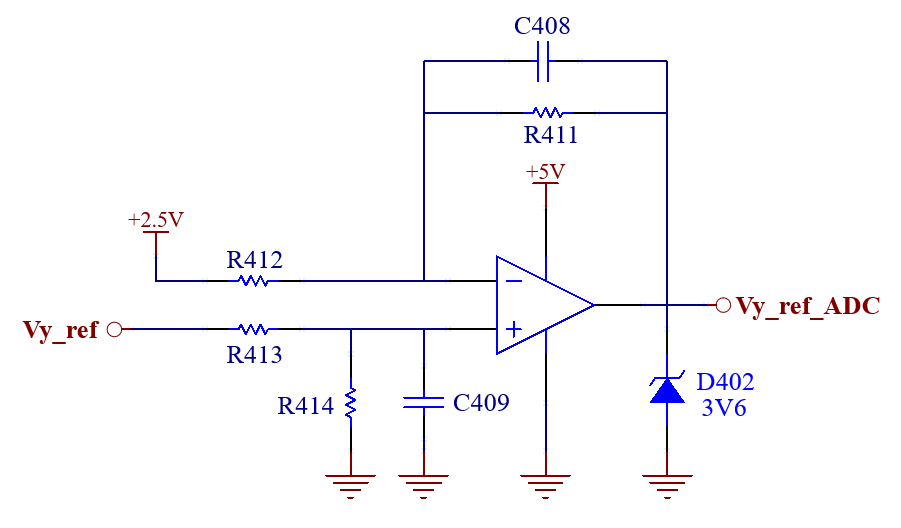
\includegraphics[scale=0.8]{Circuito-ref-posicion_dig.png}
	\caption{Circuito acondicionador para referencia de posición.}
	\label{fig:circuito-ref-posicion}
\end{figure}

\colorbox{red}{Cambiar nombre a imagen Vyref y VyrefADC} - listo
%
%Como se ve en la expresión \ref{eq_vyref_vs_yg}, la señal tiene un punto de operación de $3.4\:V$. Por lo tanto si se implementa un circuito de acondicionamiento que le reste este valor, se obtiene una señal apta para el ADC.
%  
%  
%Se utiliza el circuito mostrado en la figura \ref{fig:circuito-ref-posicion}. A la señal de entrada se le resta el punto de operación de $3.4\:V$, para lograr señales que van desde $0.56\:V$ a $1.29\:V$. Luego, dentro del microcontrolador, se debe asignar cada valor leído por el ADC a una distancia de separación deseada ($Y_{ref}$) utilizando la ganancia del estimador analógico según la expresión \ref{eq_y-ref-dig}.
 
A continuación se analiza la salida de este circuito en función de sus entradas para diseñar los valores de sus componentes. Para simplificar el análisis se define:

\begin{equation*} 
	Z=\frac{1}{sc_{408}}//R_{411}=\frac{1}{sc_{409}}//R_{414}
\end{equation*}

Por lo tanto, la salida del circuito se puede expresar como:

\begin{equation*} 
	Vy_{ref_{ADC}}=\frac{Z}{Z+R_{413}}(1+\frac{Z}{R_{412}})Vy_{ref}-\frac{Z}{R_{412}}*2.5\:V
\end{equation*}

Si se considera que $R_{412}=R_{413}$ resulta:

%y que $2.5\:V$ es una señal continua se obtiene:
\begin{equation*} 
	Vy_{ref_{ADC}}=\frac{Z}{R_{412}}Vy_{Ref}-\frac{Z}{R_{412}}*2.5\:V
\end{equation*}


Como se desea ganancia unitaria, se define que $R_{411}=R_{412}$ y se obtiene:

\begin{equation*} 
	Vy_{ref_{ADC}}=\frac{1}{1+sC_{408}R_{411}}(Vy_{Ref}-2.5\:V)
\end{equation*}

%\begin{equation*} 
%	\frac{Vy_{ref_{ADC}}}{Vy_{Ref}}=\frac{R_{411}*(R_{413}+R_{414})}{R_{413}*(R_{411}+R_{412})}*\frac{sC_{408}(R_{411}//R_{412})+1}{(sC_B(R_{413}//R_{414})+1)*(sC_{408}R_{411}+1)}
%\end{equation*}

Por lo tanto, para obtener una frecuencia de corte para el filtro de $1\:kHz$ se elige $R_{411}=10\:k\Omega$ y resulta $C_{408}=16\:nF$. De esta forma, se obtiene que $R_{412}=R_{413}=R_{414}=10\:k\Omega$ y que $C_{409}=16\:nF$.


\subsubsection{Componente  alterna de corriente del electroimán}

 Para obtener solamente la componente alterna de la corriente, se implementa un circuito con característica pasa-banda que se muestra en la figura \ref{fig:componente-corriente-alterna}. La frecuencia de corte inferior  es de $100\:Hz$, con el objetivo de eliminar el valor medio de señal. Por otro lado, la superior es de $12\:kHz$, que actúa como filtro anti-solapamiento. Luego, la salida es amplificada con una ganancia de 50 veces, según se calculó en la sección \ref{sec_adaptacion_señal_vh_ADC} y se agrega un punto de operación de $2.5\:V$.


\begin{figure}[H]
	\centering
	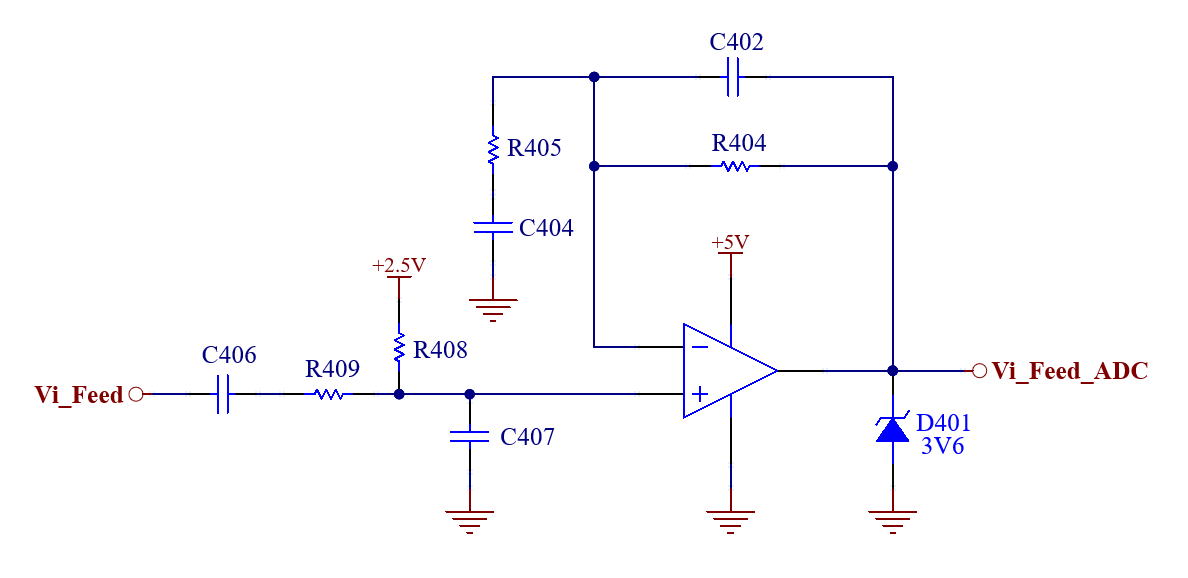
\includegraphics[scale=0.5]{Componente-corriente-alterna_dig.png}
	\caption{ Circuito acondicionador para componente alterna de corriente del electroimán.
	}
	\label{fig:componente-corriente-alterna}
\end{figure}

Para resolver este circuito se plantea:

\begin{equation*} 
	Z_1=\frac{1}{sC_{404}}+R_{405}=\frac{1}{sC_{406}}+R_{409}
\end{equation*}

\begin{equation*} 
	Z_2=\frac{1}{sC_{402}}//R_{404}=\frac{1}{sC_{407}}//R_{408}
\end{equation*}

La salida en función de sus entradas resulta:

\begin{equation*} 
	V_{IfeedADC} =\frac{Z_2}{Z_1}*Vi_{feed}+2.5\:V
\end{equation*}

\begin{equation*} 
	V_{IfeedADC} =\frac{sC_{404}R_{404}}{(1+sC_{402}R_{404})(1+sC_{404}R_{405})}*Vi_{feed}+2.5\:V
\end{equation*}

Para lograr la frecuencia de corte inferior de $100\:Hz$ es necesario definir correctamente los valores de los componentes correspondientes a $Z_1$. Para ello, se plantea la siguiente ecuación:

\begin{equation*} 
	100\:Hz=\frac{1}{2\pi C_{404}R_{405}}
\end{equation*}

Se elige $R_{405}=1\:k\Omega$ por lo que resulta $C_{404}=1.6\:\mu F$. De esta forma se obtiene $R_{409}=1\:k\Omega$ y $C_{406}=1.6\:\mu F$.

Debido a la acción del cero en el origen, la ganancia del circuito ira en aumento hasta alcanzar la frecuencia del primero polo ubicado en $100\:Hz$. Una vez alcanzado, la ganancia permanecerá constante. Ese valor es la ganancia resultante en la banda de paso. Como se desea que sea de 50, se plantea la siguiente ecuación:

\begin{equation*} 
	\frac{1}{2\pi C_{404}R_{404}}=\frac{100\:Hz}{50}
\end{equation*}

Por lo tanto, resulta $R_{404}=50\:K\Omega$. De esta forma se obtiene $R_{408}=50\:K\Omega$

Finalmente, para lograr una frecuencia de corte superior de $12\:KHz$ se plantea:

\begin{equation*} 
	12\:kHz=\frac{1}{2\pi C_{402}R_{404}}
\end{equation*}

Por lo tanto, se obtiene $C_{402}=270\:pF$. De esta forma resulta $C_{407}=270\:pF$.



%\begin{equation*} 
%	Z_1=Z_{C_{402}}//R_{404}
%\end{equation*}
%
%\begin{equation*} 
%	Z_2=Z_{C_{404}}+R_{405}
%\end{equation*}
%
%\begin{equation*} 
%	Z_3=Z_{C_{407}}//R_{408}
%\end{equation*}
%
%\begin{equation*} 
%	Z_4=Z_{C_{406}}+R_{409}
%\end{equation*}
%
%Luego con estas impedancias se plantean las ecuaciones para los nodos:
%
%\begin{equation*} 
%	V^- = \frac{Z_3}{Z_3+Z_4}
%\end{equation*}
%
%\begin{equation*} 
%	V^+ = \frac{Z_2}{Z_2+Z_1}
%\end{equation*}
%
%Adoptando $Vd=V^+-V^-$, planteando la cadena de avance($A_w$),  realimentacion($H$), $G^-$ y suponiendo que $A_w>>1/H$ se puede expresar la ecuacion final como:
%
%\begin{equation*} 
%	V_{IfeedADC} = \frac{Z_2}{Z_2+Z_1}*\frac{Z_3+Z_4}{Z_3} *Vi_{feed}
%\end{equation*}
%
%Considerando que $Z_4+Z_3 = Z_2+Z_1$ y simplificando se obiene que: 
%
%\begin{equation*} 
%	V_{IfeedADC} = \frac{Z_2}{Z_3}*Vi_{feed}=\frac{Z_{C_{404}}+R_{405}}{Z_{C_{407}}//R_{408}}*Vi_{feed}
%\end{equation*}
%
%Que es igual a:
%
%\begin{equation*} 
%	V_{IfeedADC} = \frac{(sC_{404}R_{405}+1)*(sC_{407}R_{408}+1)}{SC_{404}R_{408}}*Vi_{feed}
%\end{equation*} 


\subsubsection{Componente continua de corriente del electroimán}

 Para obtener la componente de continua se utiliza un filtro pasa-bajos con frecuencia de corte en $100\:Hz$. Se eligió esta frecuencia para que se ubique por lo menos una década por debajo de la frecuencia fundamental de la onda triangular. La implementación circuital puede observarse en la figura \ref{fig:componente-corriente-continua}


\begin{figure}[H]
	\centering
	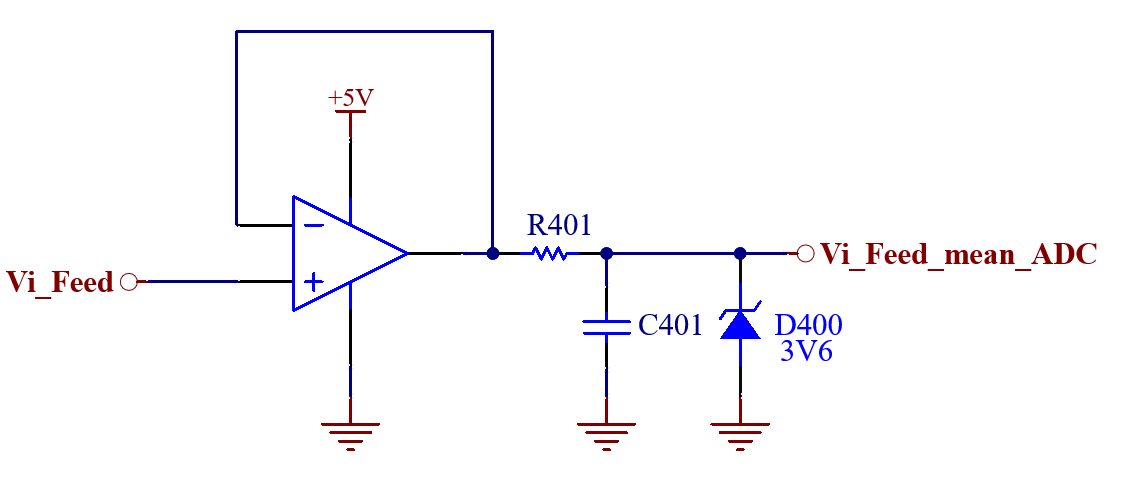
\includegraphics[scale=0.5]{Componente-corriente-continua_dig.png}
	\caption{Circuito acondicionador para componente continua de corriente del electroimán.
	}
	\label{fig:componente-corriente-continua}
\end{figure}

La señal de salida puede ser expresada en función de su entrada como:

\begin{equation*}
	Vi\_Feed\_mean\_ADC=\frac{1}{1+sC_{401}R_{401}}*Vi\_Feed
\end{equation*}
Por lo tanto, como se desea una frecuencia de corte de $100\:Hz$ se plantea la siguiente ecuación:
\begin{equation*} 
	\frac{1}{2\pi C_{401}R_{401}}=100\:Hz
\end{equation*}

Al elegir una resistencia $R_{401}=10\:k\Omega$ resulta en $C_{401}=160\:nF$


\subsection{Circuitos de acondicionamiento de señales para el DAC}

 Para convertir los valores digitales de la estimación de posición y de la compensación al dominio analógico, se utiliza el DAC del microcontrolador. El DAC utilizado entrega una tensión de salida que puede variar entre $0\:V$ y $3.3\:V$, y se actualiza con una frecuencia mínima de $3.5\:kHz$ como se mencionó en la sección \ref{sec_adquisicion_y_procesamiento}. Se agrega circuitería de filtrado, ganancia y protección en las salidas del DAC para hacerlas aptas para ingresar a las etapas analógicas.
 
\subsubsection{Salida del compensador}

La salida de la etapa de compensador digital es convertida en una señal analógica por el DAC y luego de esta etapa de adaptación ingresa a la etapa de controlador de corriente. Como el controlador de corriente funciona con tensiones de referencia de hasta $5\:V$ en su entrada y el compensador fue diseñado teniendo en cuenta este nivel de tensión, se agrega una ganancia por firmware de $0.66$, mapeando así los $5\:V$ a $3.3\:V$, que es la máxima tensión entregada por el DAC. Luego, para compensar esta ganancia y no afectar a la transferencia de la planta, se la afecta por un factor de $\frac{5V}{3.3V}$ por medio del circuito de acondicionamiento. Además, la salida del DAC es filtrada con un filtro pasa bajos con frecuencia de corte en $1.75\:kHz$ para eliminar los saltos de tensión que provoca el ROC.

De esta forma, se logra convertir correctamente la señal digital en analógica. En la figura \ref{fig:DAC-compensador} se muestra la implementación del circuito.

\begin{figure}[H]
	\centering
	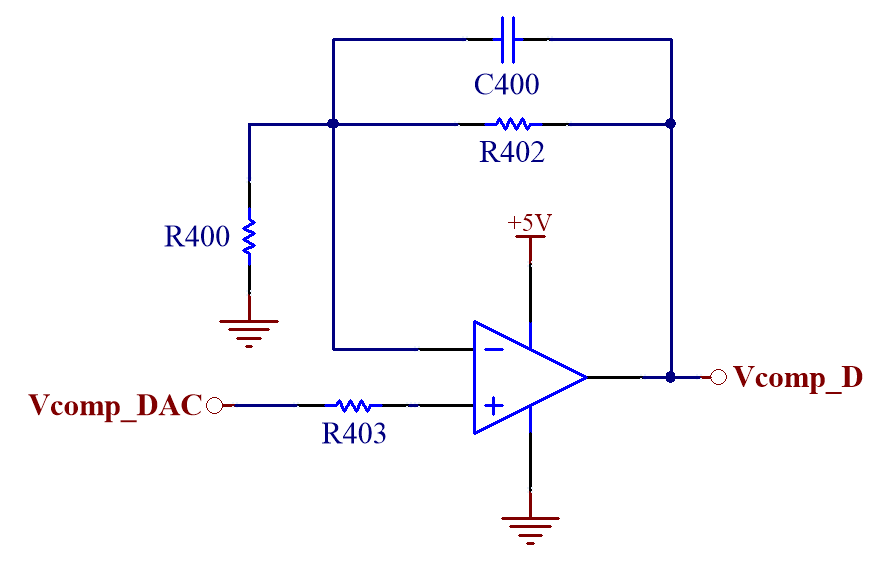
\includegraphics[scale=0.5]{DAC-compensador_dig.png}
	\caption{Circuito acondicionador para la salida del DAC correspondiente al compensador.}
	\label{fig:DAC-compensador}
\end{figure}

La salida del circuito en función de su entrada es:

\begin{equation*} 
	V_{comp\_D}=(\frac{R_{402}}{R_{400}} *\frac{1}{1+sC_{400}R_{402}}+1)*V_{comp\_DAC}
\end{equation*}

Para conseguir una ganancia en continua de  $\frac{5V}{3.3V}$ se plantea:

\begin{equation*} 
	\frac{R_{402}}{R_{400}} +1 = \frac{5V}{3.3V}
\end{equation*}

Por lo tanto, se elige $R_{400}=10\:k\Omega$ y resulta $R_{402}=5\:k\Omega$. 

Para que la frecuencia de corte del filtro se encuentre en $1.75\:kHz$, se plantea:

\begin{equation*} 
	\frac{1}{2\pi C_{400}R_{402}}=1.75\:kHz
\end{equation*}

De esta forma, se obtiene $C_{400}=18\:nF$. 

\colorbox{red}{Aclaramos para que se usa R403?} capaz la sacamos de la imgen jeje	- listo


\subsubsection{Salida del estimador}

La salida del estimador digital se obtiene a través del DAC para poder observarla mediante un osciloscopio en el PCB. Para diseñar la etapa de adaptación se utilizan los mismos criterios que para el circuito \ref{fig:DAC-compensador}. Por lo tanto, el circuito utilizado se muestra en la figura \ref{fig:DAC-estimador} cuyos valores para los componentes resultan: $C_{403}=18\:nF$, $R_{407}=5\:k\Omega$ y $R_{406}=10\:k\Omega$.

\begin{figure}[H]
	\centering
	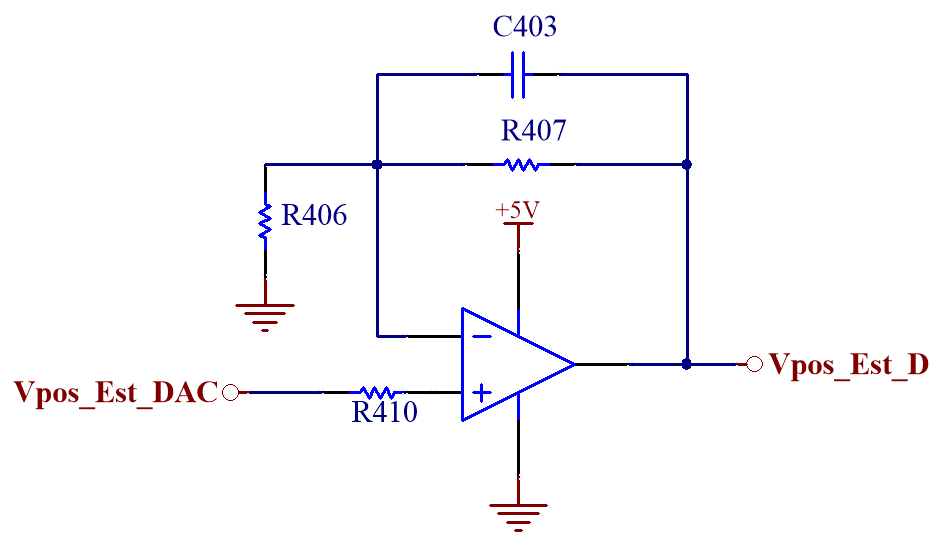
\includegraphics[scale=0.5]{DAC-estimador_dig.png}
	\caption{Circuito acondicionador para la salida del DAC correspondiente al estimador digital.}
	\label{fig:DAC-estimador}
\end{figure}

\colorbox{red}{Aclaramos para que se usa R410?}

\section{Diseño del controlador digital}

En esta sección se realiza el diseño del controlador digital teniendo en cuenta los aspectos mencionados en la sección  \ref{consideraciones_sistemas_discretos} sobre el trabajo con sistemas discretos. En la figura asdds se muestra un diagrama general del sistema de control.

Este controlador que se va a diseñar tiene como entrada la señal de referencia de posición $Y_{ref}$ calculada en \ref{sec_referencia_pos} y se realimenta la señal de posición estimada $Y_g$.


\subsection{Transferencias de la planta y del controlador de corriente}

 Para el análisis del compensador digital se parte de las transferencias de la planta $G_P(s)$ (\ref{eq_transferencia_planta_m}) y del controlador de corriente $G_{iL}(s) $ (\ref{eq_TLC-cc}) en el dominio analógico para una masa de $30 \:kg$.

\begin{equation} 
	\begin{aligned}
		G_T(s)[M=30kg]&=G_P(s)*G_{iL}(s)&=\frac{-87.7}{\ (s-70)\ (s+70)\ (s+12.17)}\\
	\end{aligned}
\end{equation}



Para incluir el efecto del ROC a esta transferencia se aplica la transformada z por el método de invarianza al impulso. 

\begin{equation*}
	G_T(z)=Z\{\frac{(1-e^{-s*T_s})}{s}*G_T(s)\}=(1-z^{-1})*Z\{\frac{G_T(s)}{s}\})
\end{equation*}

 Como se mencionó en la sección \ref{sec_adquisicion_y_procesamiento}, se utiliza una frecuencia de muestreo  $F_s=3.5\:kHz$. Por lo tanto, se obtiene:

\begin{equation} 
	G_T(z)[M=30\:kg] =\frac{-3.2057*10^{-10}(z+3.729)(z+0.2677)}{(z-0.9966)(z-0.9806) (z-1.02)}
\end{equation}

Luego, se utiliza la transformada bilineal ($z=\frac{1+\frac{wT_s}{2}}{1-\frac{wT_s}{2}}$) para obtener una transferencia en el dominio analógico de la variable $w$. Considerando $T_s=1/F_s$:

\begin{equation} \label{eq_Gtotal_w_m30}
	\resizebox{.8\hsize}{!}
	{
		$G_T(w)[M=30\:kg]\ \ =\frac{-8.0207*10^{-11}(w-1.238*10^4)(w-7143)(w+1.237*10^4)}{\ (w-70)\ (w+70)\ (w+12.17)}$
	}
\end{equation}


Con las expresiones en $[w]$ es posible diseñar un controlador utilizando técnicas de diseño en el dominio analógico y luego transformarlo al digital nuevamente con la transformada bilineal inversa.



\subsection{Diseño del compensador}

Se decide usar la misma estrategia utilizada en el compensador analógico, planteando dos lazos de realimentación: uno interno y otro externo. El primero con el objetivo de estabilizar la planta y el segundo para mejorar la respuesta temporal del sistema. Por lo tanto, se plantea el diagrama en bloques de la figura \ref{fig:diag-en-bloques-comp_digital}.

\begin{figure}[H]
	\centering
	\scalebox{0.8}{\tikzset{%
	buffer/.style={
		draw,
		shape border rotate=270,
		regular polygon,
		regular polygon sides=3,
		fill=blue!20,
		node distance=2cm,
		minimum height=4em
	}
}

\tikzstyle{block} = [draw, fill=blue!20, rectangle, 
minimum height=2.5em, minimum width=3em]

%Acá se define eñ diagrama en bloques completo
\begin{tikzpicture}[auto, node distance=1cm,>=latex']
	% We start by placing the blocks
	\node [input, name=input] {};
	\node [buffer, right=of input](F){F};
	\node [sum, right of=F, node distance=1.5cm] (suma_externa) {+};
	\node [block, right=of suma_externa] (externo) {$G_{ext}(w)$};
	\node [sum, right=of externo] (suma_interna) {+};
	\node[block, right=of suma_interna] (interno) {$G_c(w)$};
	\node [block, right=of interno] (gil) {$G_{IL}(w)$};
	\node [block, right=of gil] (planta) {$G_p(w)$};
	\node [coordinate, below=of interno] (realimentacion_interna) {$H_{estim}(w)$};
	
	\node [coordinate, below=2cm of externo] (realimentacion_externa) {$H_{estim}$};
%	
%	\node [block, right of=suma] (amplificador) {$A(s)$};
	\node [output, right of=planta, node distance=3cm] (output) {};
%	\node [block, below of=amplificador] (realimentacion) {$H(s)$};
%	
%	
%	% Once the nodes are placed, connecting them is easy. 
	\draw [draw,->] (input) -- node[pos=0.2]{$V_{y_{ref}}$} (F);
	\draw [draw,->] (F) -- node[pos=0.9]{$+$}(suma_externa);
	\draw [draw,->] (suma_externa) -- (externo);
	\draw [draw,->] (externo) -- node[pos=0.95]{$+$} (suma_interna);
	\draw [draw,->] (suma_interna) -- (interno);
	\draw [draw,->] (interno) -- (gil);
	\draw [draw,->] (gil) -- (planta);
	\draw [draw,->] (planta) -- node[name=y]{$Y_g$} (output);
%	\draw [draw,->] (amplificador) -- node[name=y]{$V_{deriv}$} (output);
	\draw [-] (y) |- (realimentacion_interna);
	\draw [->] (realimentacion_interna) -|  node[pos=0.99]{$-$} (suma_interna);
	\draw [-] (y) |- (realimentacion_externa);
	\draw [->] (realimentacion_externa) -|  node[pos=0.99]{$-$} (suma_externa);
\end{tikzpicture}}
	\caption{Diagrama en bloques de estrategia de compensación propuesta.}	\label{fig:diag-en-bloques-comp_digital}
\end{figure}

\colorbox{red}{aclaramos que se considera H=1?}
En el diagrama en bloques de la figura \ref{fig:diag-en-bloques-comp_digital} la realimentación es unitaria ya que el algoritmo encargado de la estimación de distancia de entrehierro entrega directamente el valor estimado.

\subsection{Diseño del lazo de realimentación interno}

En esta sección se diseña el control del lazo de realimentación interno, que está compuesto por las etapas mostradas en la figura \ref{fig:diag-interno_dig}. Donde $G_c$ corresponde a la transferencia del compensador que se desea diseñar, $G_{T}$ a la transferencia del controlador de corriente junto con la de la planta. Todas las transferencias pertenecen al dominio de la variable [w].

\begin{figure}[H]
	\centering
	\tikzset{%
	buffer/.style={
		draw,
		shape border rotate=270,
		regular polygon,
		regular polygon sides=3,
		fill=blue!20,
		node distance=2cm,
		minimum height=4em
	}
}

\tikzstyle{block} = [draw, fill=blue!20, rectangle, 
minimum height=2.5em, minimum width=3em]

%Acá se define eñ diagrama en bloques completo
\begin{tikzpicture}[auto, node distance=1.5cm,>=latex']
	% We start by placing the blocks
	\node [input, name=input] {};
	\node [sum, right of=input, node distance=1.5cm] (suma_interna) {+};
	\node[block, right=of suma_interna] (interno) {$G_c$};
	\node [block, right=of interno] (gil) {$G_{IL}$};
	\node [block, right=of gil] (planta) {$G_p$};
	\node [block, below=of gil] (realimentacion_interna) {$H_{estim}$};
	
	
%	\node [block, right of=suma] (amplificador) {$A(s)$};
	\node [output, right of=planta, node distance=3cm] (output) {};
%	\node [block, below of=amplificador] (realimentacion) {$H(s)$};
%	
%	
%	% Once the nodes are placed, connecting them is easy. 
%	\draw [draw,->] (input) -- node[pos=0.2]{$V_{y_{ref}}$} (F);
	\draw [draw,->] (input) -- node[pos=0.2]{$V_{ref_c}$} node[pos=0.9]{$+$}(suma_interna);

	\draw [draw,->] (suma_interna) -- node{$Ve_{int}$} (interno);
	\draw [draw,->] (interno) -- node{$V_{IL{ref}}$} (gil);
	\draw [draw,->] (gil) -- node{$I_L$} (planta);
	\draw [draw,->] (planta) -- node[name=y]{$Y_g$} (output);
%	\draw [draw,->] (amplificador) -- node[name=y]{$V_{deriv}$} (output);
	\draw [->] (y) |- (realimentacion_interna);
	\draw [->] (realimentacion_interna) -| node[pos=0.25]{$V_{estim}$}  node[pos=0.99]{$-$} (suma_interna);
%	\draw [->] (y) |- (realimentacion_externa);
%	\draw [->] (realimentacion_externa) -| node[pos=0.25]{$V_{estim}$} node[pos=0.99]{-} (suma_externa);
\end{tikzpicture}
	\caption{Diagrama en bloques del lazo de compensación interno.}	\label{fig:diag-interno_dig}
\end{figure}

\colorbox{red}{ver si cambiamos lso nombres de las señales}

La transferencia de lazo cerrado ($TLC_{interna}$) del diagrama \ref{fig:diag-interno_dig} queda definida como:

\begin{equation}
	TLC_{interna}=\frac{Y_g[m]}{V_{ref_c}[V]}=\frac{G_c*G_T}{1+G_c*G_T}
\end{equation}

A continuación se analiza la estabilidad de la planta considerando una masa $M=30\:kg$ y se diseña el bloque del compensador interno $G_c(w)$ para lograr estabilizarla. Luego, se verificará la estabilidad con este mismo compensador para una masa $M=1\:kg$, que corresponde a la mínima con la que trabaja el sistema.

\subsubsection{Análisis de estabilidad}

 Para el análisis de la estabilidad de la planta se debe obtener la transferencia de lazo abierto total $GH_T(w)=G_T(w)*H(w)$. Se tiene la transferencia de la ganancia de avance $G_{T}(w)$ para una masa de $30\:kg$ calculada en \ref{eq_Gtotal_w_m30} y la del lazo de realimentación $H(w)=1$. A partir de ellas se obtiene la transferencia a lazo abierto total $GH_{T}(w)=G_{T}(w)*H(w)$ mostrada en la ecuación \ref{eq:GtHW}.

\colorbox{red}{Ver si ya mencionamos que H=1. Si ya lo mencionamos, redactar lo de arriba para que quede bien} --> ahí traté de acomodarlo. arriba puse que la realimentación es unitaria.
 
\begin{equation}
	\label{eq:GtHW}  
	GH_{T}(w)=\frac{-8.5*10^{-11}(w-1.21*10^4)(w-7000)(w+1.21*10^4)}{\ (w-70)\ (w+70)\ (w+12.17)} 
\end{equation} 


 A continuación se procede a analizar la respuesta en frecuencia de $GH_{T}(w)$ y a diseñar un compensador adecuado. Luego, al igual que para el compensador analógico, se verificará la estabilidad para la mínima masa  con la  que trabaja el sistema.
 
Para comenzar el análisis se considera un compensador $G_c=K$, donde K es una constante positiva. Por lo tanto, se plantea la transferencia de lazo abierto teniendo en cuenta el compensador:
 
 \begin{equation} \label{eq_GT3_dig}
 		\resizebox{.85\hsize}{!}
 	{
 	$G_c*GH_T(w)=\frac{-8.5*10^{-11}*K*(w-1.21*10^4)(w-7000)(w+1.21*10^4)}{\ (w-70)\ (w+70)\ (w+12.17)}$ 
 }
 \end{equation}
\colorbox{red}{hacer resize de la ecuacion} -> creo que ahí quedó bien

\colorbox{red}{Pasar esta expresión a lla forma de 1+w/p} -> creo que al final lo dejamos como está

 A partir de la transferencia de la ecuación  \ref{eq_GT3_dig} se  grafica el diagrama de Bode y el de Nyquist considerando $K=1$. Estos se muestran en las figuras \ref{fig:bode_digital} y \ref{fig:nyquist-lazo-abierto-digital} respectivamente.

\begin{figure}[H]
	\centering
	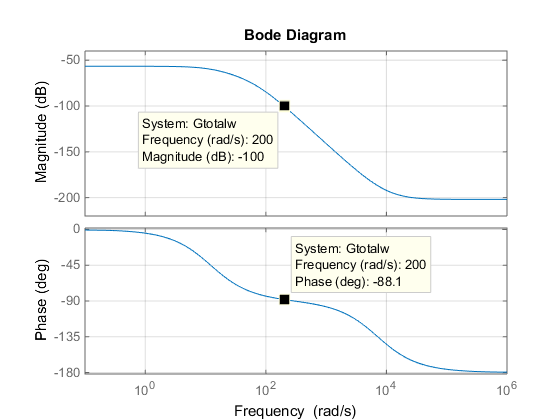
\includegraphics[scale=0.8]{diag_bode_planta_en_w.png}
	\caption{Diagrama de Bode de lazo abierto $G_c*GH_{T}(w)$ con $M=30\:kg$.}
	\label{fig:bode_digital}
\end{figure}

\begin{figure}[H]
	\centering
	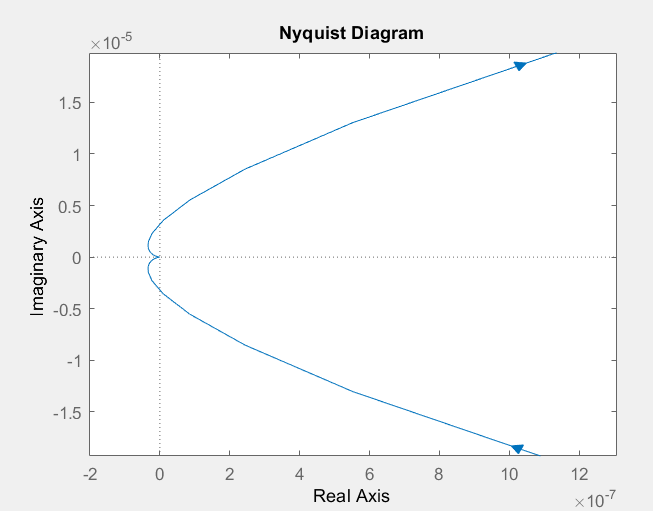
\includegraphics[scale=0.75]{Nyquist-lazo-abierto-digital.png}
	\caption{Diagrama de Nyquist de $G_c*GH_{T}(w)$ con $M=30\:kg$.}
	\label{fig:nyquist-lazo-abierto-digital}
\end{figure}

Como la transferencia de la planta $GH_T$ tiene un polo en el semiplano derecho del plano ``w'' no es posible determinar su estabilidad por medio del diagrama de Bode. Por lo tanto, se analiza la estabilidad por medio del criterio de Nyquist.

Como se observa en el diagrama en bloques de la figura \ref{fig:diag-interno_dig}, para compensar al sistema se planteó una realimentación negativa. Por lo tanto, para analizar su estabilidad según Nyquist se deben determinar la cantidad de giros (N) de $G_c*GH_T$ alrededor del punto $-1+j0$ en la figura \ref{fig:nyquist-lazo-abierto-digital} y la cantidad de polos (P) en el semiplano derecho de la función transferencia $G_c*GH_T$. El sistema resultará estable si se cumple la condición \ref{eq_condicion_Nyquist}, donde Z representa la cantidad de ceros en el semiplano derecho de $1+G_c*GH_T(w)$.

\begin{equation}\label{eq_condicion_Nyquist}
	Z=N+P=0
\end{equation}


Debido a que $GH_T$ tiene un polo en el semiplano derecho ($P=1$) y no hay giros alrededor del punto $-1+j0$ ($N=0$), resulta que $Z=1$. Por lo tanto, la transferencia de lazo cerrado ($TLC_{interna}$) presenta un comportamiento inestable. En la figura \ref{fig:nyquist-lazo-abierto-digital} se puede observar que no existe ningún valor de $K>0$ que haga que el contorno de $G_c*GH_T$ rodee el punto $-1+j0$. Por lo tanto, se propone implementar un compensador con $K<0$, para invertir el contorno de $G_c*GH_T$. Esto resulta equivalente a considerar $K>0$ y usar realimentación positiva en el lazo de control interno. De esta forma se obtiene el diagrama en bloques de la figura \ref{fig:diag-interno_dig_realimentacion_positiva}.


\begin{figure}[H]
	\centering
	\tikzset{%
	buffer/.style={
		draw,
		shape border rotate=270,
		regular polygon,
		regular polygon sides=3,
		fill=blue!20,
		node distance=2cm,
		minimum height=4em
	}
}

\tikzstyle{block} = [draw, fill=blue!20, rectangle, 
minimum height=2.5em, minimum width=3em]

%Acá se define eñ diagrama en bloques completo
\begin{tikzpicture}[auto, node distance=1.5cm,>=latex']
	% We start by placing the blocks
	\node [input, name=input] {};
	\node [sum, right of=input, node distance=1.5cm] (suma_interna) {+};
	\node[block, right=of suma_interna] (interno) {$G_c$};
	\node [block, right=of interno] (gil) {$G_{IL}$};
	\node [block, right=of gil] (planta) {$G_p$};
	\node [block, below=of gil] (realimentacion_interna) {$H_{estim}$};
	
	
%	\node [block, right of=suma] (amplificador) {$A(s)$};
	\node [output, right of=planta, node distance=3cm] (output) {};
%	\node [block, below of=amplificador] (realimentacion) {$H(s)$};
%	
%	
%	% Once the nodes are placed, connecting them is easy. 
%	\draw [draw,->] (input) -- node[pos=0.2]{$V_{y_{ref}}$} (F);
	\draw [draw,->] (input) -- node[pos=0.2]{$V_{ref_c}$} node[pos=0.9]{$+$}(suma_interna);

	\draw [draw,->] (suma_interna) -- node{$Ve_{int}$} (interno);
	\draw [draw,->] (interno) -- node{$V_{IL{ref}}$} (gil);
	\draw [draw,->] (gil) -- node{$I_L$} (planta);
	\draw [draw,->] (planta) -- node[name=y]{$Y_g$} (output);
%	\draw [draw,->] (amplificador) -- node[name=y]{$V_{deriv}$} (output);
	\draw [->] (y) |- (realimentacion_interna);
	\draw [->] (realimentacion_interna) -| node[pos=0.25]{$V_{estim}$}  node[pos=0.99]{$+$} (suma_interna);
%	\draw [->] (y) |- (realimentacion_externa);
%	\draw [->] (realimentacion_externa) -| node[pos=0.25]{$V_{estim}$} node[pos=0.99]{-} (suma_externa);
\end{tikzpicture}
	\caption{Diagrama en bloques del lazo de compensación interno con realimentación positiva.}	\label{fig:diag-interno_dig_realimentacion_positiva}
\end{figure}

La realimentación positiva se genera al sumar la señal $Y_g$ con la señal de entrada del sistema. La transferencia de lazo cerrado del diagrama en bloques ahora se define como:

\begin{equation}
	TLC_{interna}=\frac{Y_g[m]}{V_{ref_c}[V]}=\frac{G_c*G_T}{1-G_c*G_T}
\end{equation}

Siguiendo el criterio de estabilidad de Nyquist, al utilizar realimentación positiva, la cantidad de giros (N) debe analizarse alrededor del punto $1+j0$. Si estos son en sentido horario, N será positivo, caso contrario será negativo. Al variar el valor de K, es posible hacer que el punto $1+j0$ quede contenido en la zona 1 o en la zona 2 de la figura \ref{fig:nyquist-con-zonas_digital}. 

\begin{figure}[H]
	\centering
	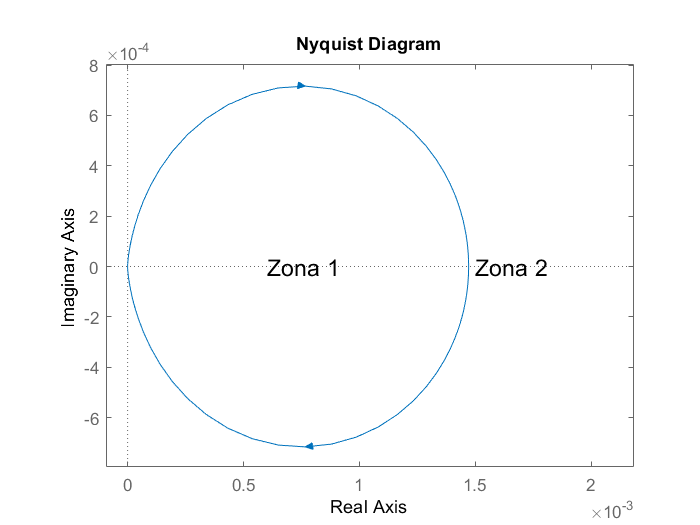
\includegraphics[scale=0.75]{Nyquist-lazo-abierto-digital-zonas.png}
	\caption{Diagrama de Nyquist con zonas marcadas.}
	\label{fig:nyquist-con-zonas_digital}
\end{figure}

Si el punto queda dentro de la zona 1, el número de giros es $N=1$. Por lo tanto, se plantea:

\begin{equation*}
	Z = N + P = 2
\end{equation*}


Si el punto queda dentro de la zona 2, el número de giros es $N=0$. Por lo tanto, se plantea:

\begin{equation*}
	Z = N + P = 1
\end{equation*}

Debido a que en ambas zonas Z resulta mayor que cero, el sistema realimentado no puede ser estabilizado con ningún valor de K. Para lograrlo se debe implementar un compensador $G_c$ que sea capaz de generar una zona en el diagrama de Nyquist donde exista un giro alrededor de $1 + j0$ en sentido antihorario de forma tal que $N=-1$ y resulte $Z=0$. Para ello, es necesario aumentar la fase para que pueda superar el valor de 0$\mathrm{{}^\circ}$. Para que esto se cumpla, el diagrama de Nyquist debe tener una forma como la  mostrada en la figura \ref{fig:nyquist-deseado-dig}.

\begin{figure}[H]
	\centering
	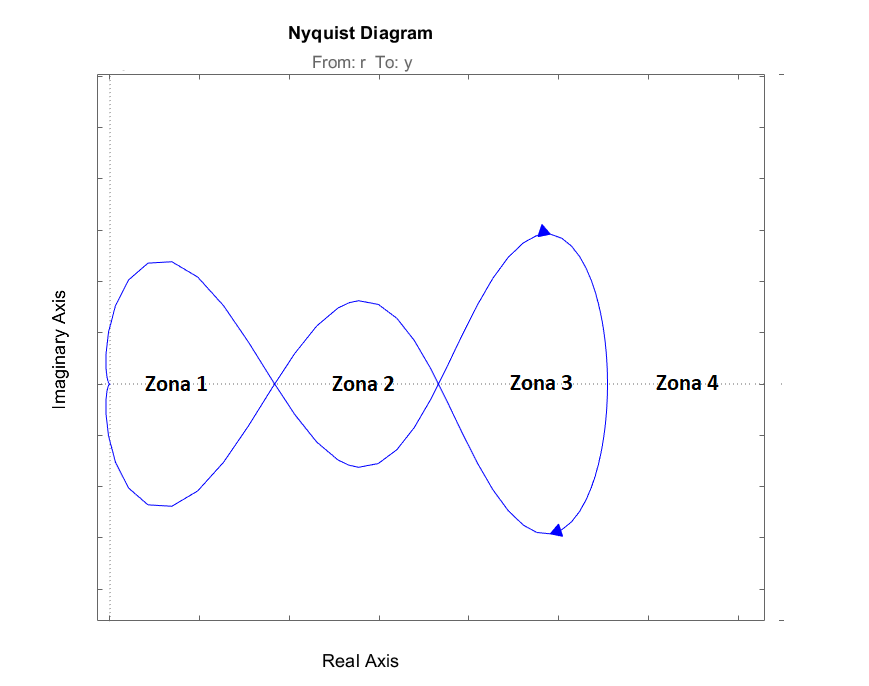
\includegraphics[scale=0.7]{Nyquist-deseado-dig.png}
	\caption{Diagrama de Nyquist deseado.}
	\label{fig:nyquist-deseado-dig}
\end{figure}

De esta manera se identifican cuatro zonas en las que puede estar ubicado el punto $1+j0$. Sin embargo, solo en la zona 2 se genera un giro en sentido antihorario ($N=-1$) como es deseado, por lo que resulta:

\begin{equation*}
	Z = N + P = 0
\end{equation*}

%Para lograr el comportamiento del sistema como en la figura 	\ref{fig:nyquist-deseado-analog} se debe tener en cuenta que el m\'{o}dulo de la transferencia de lazo abierto en el primer cruce de la fase por 0$\mathrm{{}^\circ}$ debe ser mayor a $0\:dB$ y, en el segundo cruce, menor. Para ello, se propone implementar un compensador por adelanto de fase.

A continuación se diseñará el compensador $G_c$ para lograr que el diagrama de Nyquist tenga la forma deseada y así, estabilizar el sistema.

\subsubsection{Diseño del compensador}

Para lograr el comportamiento del sistema como en la figura 	\ref{fig:nyquist-deseado-dig} se utilizará una estrategia de compensación por adelanto de fase. Esta consiste en observar el diagrama de bode de la figura \ref{fig:bode_digital} y elegir una frecuencia en la que se desee aumentar la fase para lograr la estabilidad. Se debe tener en cuenta que el módulo de la transferencia de lazo abierto en el primer cruce de la fase por 0$\mathrm{{}^\circ}$ debe ser mayor a $0\:dB$ y, en el segundo cruce, menor. 

De esta forma, al observar la figura \ref{fig:bode_digital} se decide generar un adelanto de fase de por lo menos 100° en la frecuencia $200\:r/s$. Esto se logra mediante el uso de un compensador compuesto por dos redes de adelanto de fase de 65$\mathrm{{}^\circ}$ cada una. 

Una red de adelanto de fase está compuesta por un polo ($W_p$) y un cero ($W_c$), de manera que el cero se encuentra a una frecuencia menor que el polo, permitiendo un aumento de fase a la frecuencia deseada $W_0$. Su transferencia es la siguiente:

\begin{equation} \label{eq_tf_adelanto_dig}
	G_{af}(w)=\alpha*\frac{(w + W_c)}{(w + W_p)}
\end{equation}

\noindent De esta forma, las ecuaciones de diseño resultan:

\begin{equation*}
	\begin{aligned}
		&W_0 =200\:r/s\\
		&{\varphi }_{max} =65\textrm{°}\\
		&\alpha =\frac{1+sen({\varphi }_{max})}{1-sen{(\varphi }_{max})}=20.346\\
		&W_c =\frac{W_0}{\sqrt{\alpha }}=\ 44.3\:r/s\\
		&W_p =\sqrt{\alpha }*W_0=902.1\: r/s\\
	\end{aligned}
\end{equation*} 
\noindent Finalmente, agregando una ganancia K y considerando las dos redes de adelanto de fase, se llega a la transferencia del controlador:

\begin{equation}  
	G_c(s)=K*{[20.346*\frac{(s+44.3)}{(s+902.1)}]}^2
	\label{eq:transferencia-del-compensador}
\end{equation} 

En la figura \ref{fig:bode-compensado-para-k-1} se muestra el diagrama de bode de ${GH}_T(w)*G_c(w)$ con $K=1$. Se puede observar que la ganancia $K$ puede adoptar valores desde $64\:dB$ hasta $88.6\:dB$. Al considerar que el sistema debe soportar una masa variable entre $1\:kg$ y $30\:kg$, y que la ganancia de la transferencia de la planta para $1\:kg$ es de $5.5$ veces ($14\:dB$) mayor que para $30\:kg$, se debe adoptar una ganancia del compensador que mantenga la estabilidad para estos dos casos. Es decir, la ganancia m\'{i}nima es de $64\:dB$ y la m\'{a}xima es de $88.6\:dB - 14\:dB = 74.6\:dB$. Por lo tanto, se elige que el cruce por cero de la ganancia se encuentre ahora en $88\:rad/s$, lo que significa que $K=68.4\:dB\ \equiv \ 2630\:veces$.

\begin{figure}[H]
	\centering
	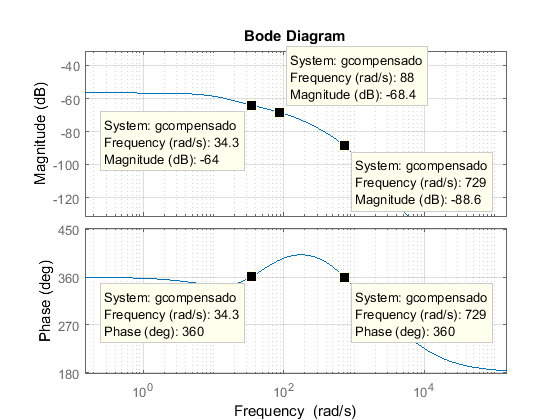
\includegraphics[scale=0.85]{Bode-compensado-para-k-1.png}
	\caption{Diagrama de Bode de $GH_T(w)*G_c(w)$ para $K=1$ y $M=30\:kg$.}
	\label{fig:bode-compensado-para-k-1}
\end{figure}
 
En la figura \ref{fig:bode-compensado-para-k-2630} se muestra el diagrama de Bode al considerar la ganancia del compensador. En ella se puede observar que se  cumple con el criterio de estabilidad, puesto que en el primer cruce por 0°, la magnitud es mayor a $0\:dB$ y en el segundo cruce, menor. Además, en la figura \ref{fig:nyquist-para-k-2630} se grafica el diagrama de Nyquist para el sistema con el compensador. En él se puede ver que el punto $1+j0$ queda dentro de la zona en la que $N=-1$, que resulta en $Z=0$.

\begin{figure}[H]
	\centering
	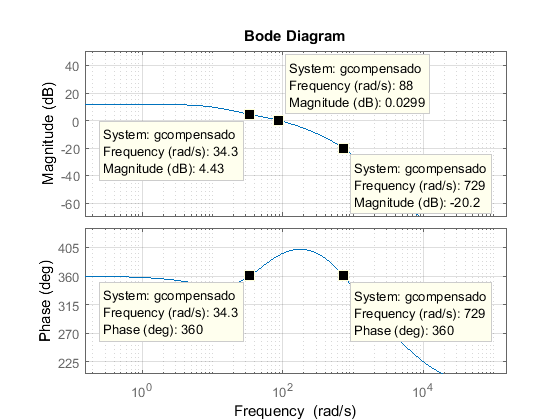
\includegraphics[scale=0.75]{Bode-compensado-para-k-2630.png}
	\caption{Diagrama de Bode de $GH_T(w)*G_c(w)$ para $K=2630$ y $M=30\:kg$.}
	\label{fig:bode-compensado-para-k-2630}
\end{figure}

\begin{figure}[H]
	\centering
	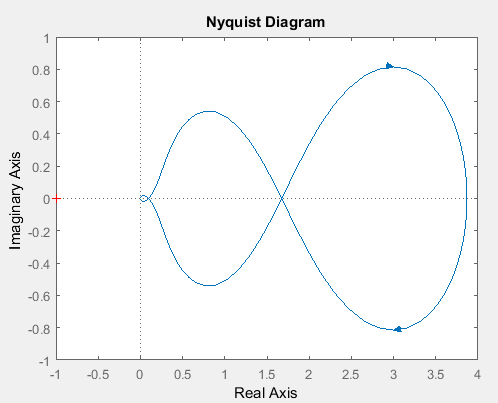
\includegraphics[scale=0.55]{Nyquist-para-k-2630.png}
	\caption{Diagrama de Nyquist de $GH_T(w)*G_c(w)$ para $K=2630$ y $M=30\:kg$.}
	\label{fig:nyquist-para-k-2630}
\end{figure}

\subsubsection{Análisis de estabilidad con masa mínima}


Se verifica la estabilidad del sistema  para el caso en que la masa sea de $1\:kg$ con el compensador previamente diseñado. Para ello, se analizan los diagramas de Bode y Nyquist mostrados en las figuras \ref{fig:bode-para-M-1Kg} y \ref{fig:nyquist-para-M-1Kg}. A partir de ellos, es posible verificar que el sistema resulta estable para todo el rango de masas en el que opera el sistema. Sin embargo, se puede observar que el margen de fase es menor que 45°, por lo que el sistema puede presentar un transitorio con oscilaciones amortiguadas. A raíz de esto, se propone implementar un lazo de control externo que permita mejorar dicha respuesta.


\begin{figure}[H]
	\centering
	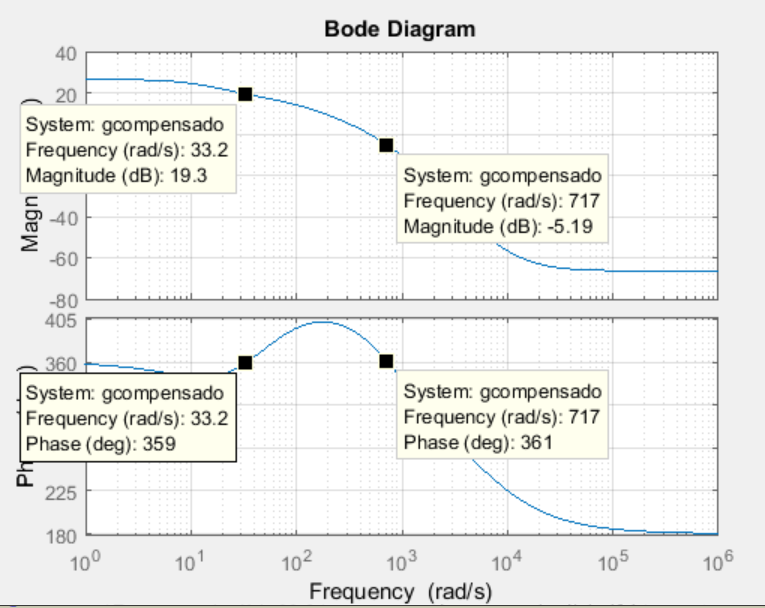
\includegraphics[scale=0.85]{Bode-para-M-1Kg.png}
	\caption{Diagrama de Bode de $GH_T(w)*G_c(w)$ para $M=1\:kg$.}
	\label{fig:bode-para-M-1Kg}
\end{figure}

\begin{figure}[H]
	\centering
	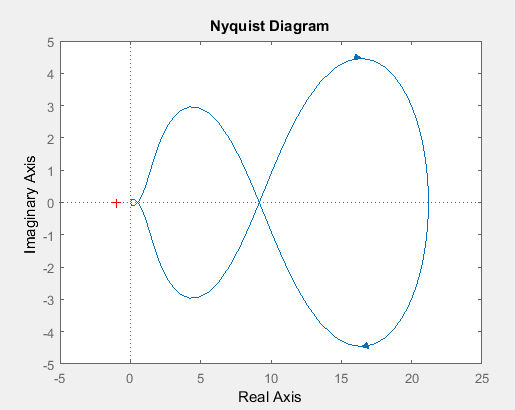
\includegraphics[scale=0.6]{Nyquist-para-M-1Kg.png}
	\caption{Diagrama de Nyquist de $GH_T(w)*G_c(w)$ para $M=1\:kg$.}
	\label{fig:nyquist-para-M-1Kg}
\end{figure}

\subsubsection{Transferencia de lazo cerrado}

Finalmente se puede expresar la función transferencia del lazo de control interno como:
%
%-3.6301e05 (s+1000) (s+44.3)^2
%------------------------------------------------------------------
%(s+304.3) (s+115.6) (s^2 + 44.84s + 2588) (s^2 + 2352s + 1.498e06)


\begin{equation}
	TLC_{interna}(w)=\frac{Y_g}{V_{ref_c}}=\frac{G_c*G_T}{1-G_c*G_T}
	%	\frac{-3.6301*}{den}
\end{equation}

Para el caso de trabajar con masa de $30\:kg$, la $TLC_{interna}$ resulta:
%
%  -8.7319e-05 (s+1.237e04) (s-1.238e04) (s-7143) (s+44.34)^2
%----------------------------------------------------------
%(s+1197) (s+471.1) (s+103.6) (s^2 + 44.34s + 2383)

\begin{equation*}
	\resizebox{.99\hsize}{!}
	{
		$
		TLC_{interna}(w)=\frac{-8.73*10^{-5} (w+1.24*10^4) (w-1.24*10^4) (w-7143) (w+44.34)^2}{(w+1197) (w+471.1) (w+103.6) (w^2 + 44.34w + 2383)}
		$
	}
\end{equation*}


Para el caso de trabajar con masa de $1\:kg$, resulta:

% -0.00047808 (s+1.237e04) (s-1.238e04) (s-7143) (s+44.34)^2
%----------------------------------------------------------
%(s+1527) (s^2 + 88.75s + 2128) (s^2 + 196.9s + 3.014e05)

\begin{equation*}
	\resizebox{.99\hsize}{!}
	{
		$
		TLC_{interna}(w)=\frac{-4.78*10^{-4} (w+1.24*10^4) (w-1.24*10^4) (w-7143) (w+44.34)^2}{(w+1527) (w^2 + 88.75w + 2128) (w^2 + 196.9w + 3.01*10^5)}	
		$
	}
\end{equation*}



En las figuras \ref{fig:ubicacion_polos_y_ceros_dig} y \ref{fig:ubicacion_polos_y_ceros_1kg_dig} se muestra la ubicación de los polos y ceros de la $TLC_{interna}$ para el caso de masa de $30\:kg$ y $1\:kg$, respectivamente. En ellas se ve que todos los polos se encuentran en el semiplano izquierdo. 

\begin{figure}[H]
	\centering
	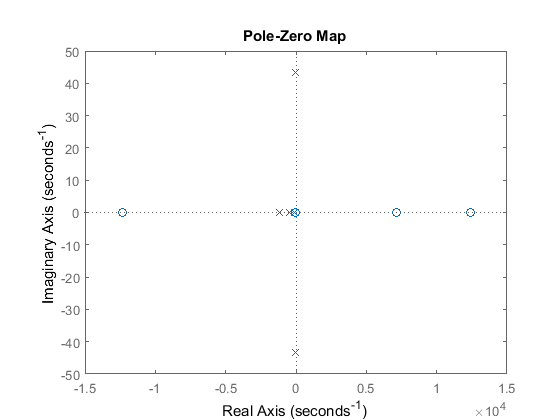
\includegraphics[scale=0.85]{ubicacion_polos_ceros_dig.png}
	\caption{Ubicación de polos y ceros de la transferencia de lazo cerrado interna con $M=30\:kg$.}
	\label{fig:ubicacion_polos_y_ceros_dig}
\end{figure}

\begin{figure}[H]
	\centering
	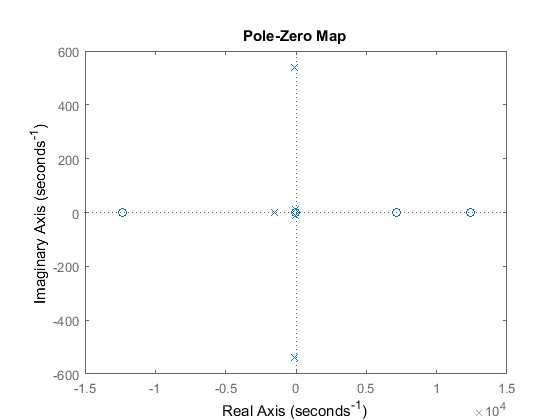
\includegraphics[scale=0.85]{ubicacion_polos_ceros_1kg_dig.png}
	\caption{Ubicación de polos y ceros de la transferencia de lazo cerrado interna con $M=1\:kg$.}
	\label{fig:ubicacion_polos_y_ceros_1kg_dig}
\end{figure}

Es importante notar que la ganancia de la transferencia de lazo cerrado en ambos casos es negativa. Esto debe tenerse en cuenta para el diseño del lazo de compensación externo.





\section{Diseño del lazo de realimentación externo}

\noindent Se plantea un lazo de realimentación externo como se muestra en la figura \ref{fig:diag-externo_dig}. 

\begin{figure}[H]
	\centering
	\tikzset{%
	buffer/.style={
		draw,
		shape border rotate=270,
		regular polygon,
		regular polygon sides=3,
		fill=blue!20,
		node distance=2cm,
		minimum height=4em
	}
}

\tikzstyle{block} = [draw, fill=blue!20, rectangle, 
minimum height=2.5em, minimum width=3em]

%Acá se define eñ diagrama en bloques completo
\begin{tikzpicture}[auto, node distance=1.5cm,>=latex']
	% We start by placing the blocks
	\node [input, name=input] {};
	\node [buffer, right=of input](F){F};
	\node [sum, right of=F, node distance=1.5cm] (suma_interna) {+};
	\node [block, right=of suma_interna] (interno) {$G_{ext}$};
	\node [block, right=of interno] (tlc_interna) {$TLC_{interna}$};
	\node [coordinate, below=of interno] (realimentacion_interna) {$H_{estim}$};
	
	
%	\node [block, right of=suma] (amplificador) {$A(s)$};
	\node [output, right of=tlc_interna, node distance=3cm] (output) {};
%	\node [block, below of=amplificador] (realimentacion) {$H(s)$};
%	
%	
%	% Once the nodes are placed, connecting them is easy. 
	\draw [draw,->] (input) -- node[pos=0.2]{$V_{y_{ref}}$} (F);
	\draw [draw,->] (F) --  node[pos=0.9]{$+$}(suma_interna);
	\draw [draw,->] (suma_interna) --node{$Ve_{ext}$} (interno);
	\draw [draw,->] (interno) -- node{$V_{ref_c}$} (tlc_interna);
	\draw [draw,->] (tlc_interna) -- node[name=y]{$Y_g$} (output);
%	\draw [draw,->] (amplificador) -- node[name=y]{$V_{deriv}$} (output);
	\draw [-] (y) |- (realimentacion_interna);
	\draw [->] (realimentacion_interna) -|   node[pos=0.99]{$-$} (suma_interna);
%	\draw [->] (y) |- (realimentacion_externa);
%	\draw [->] (realimentacion_externa) -| node[pos=0.25]{$V_{estim}$} node[pos=0.99]{-} (suma_externa);
\end{tikzpicture}
	\caption{Diagrama en bloques del lazo de compensación externo.}	\label{fig:diag-externo_dig}
\end{figure}

En el lazo de realimentación interno actúa el compensador por adelanto de fase previamente diseñado y, en el externo, se propone diseñar un controlador del tipo integral. Esto permite suavizar la respuesta al escalón del sistema y eliminar el error en régimen permanente. Para el diseño de este lazo de compensación se sigue trabajando con las transferencias en el dominio de la variable w. Finalmente se realizará la conversión de la compensación al dominio discreto.



\noindent La cadena de avance con masa de $30\:kg$ es:

\begin{equation} \label{eq_cadena_avance_integrador_dig}
	G=TLC_{interna}(w)[M=30\:kg]*G_{ext}
\end{equation}

La transferencia a lazo abierto resulta:

\begin{equation} \label{eq_lazo_abierto_externo_dig}
	GH_{externo}=TLC_{interna}(w)[M=30\:kg]*G_{ext}
\end{equation}

Se plantea un compensador del tipo integrador cuya transferencia en dominio de la variable [w] es:
\begin{equation}
	G_{ext}= \frac{K_{int}}{w}
\end{equation}


Para encontrar el valor adecuado de $K_{int}$ se grafica el lugar de raíces de la expresión \ref{eq_lazo_abierto_externo} considerando $K_{int}=1$. En la figura \ref{fig:lugar-de-raices-con-integrador_real_neg} se muestra un acercamiento del lugar de raíces en la zona del origen.


\begin{figure}[H]
	\centering
	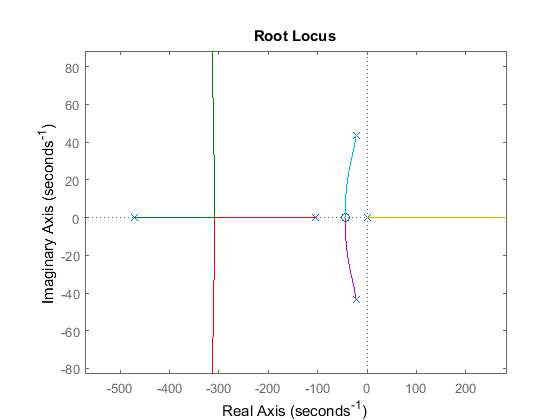
\includegraphics[scale=0.7]{Lugar-de-raices-con-integrador_real_neg.png}
	\caption{Lugar de raíces con el integrador para las transferencias en el dominio de la variable w.}
	\label{fig:lugar-de-raices-con-integrador_real_neg}
\end{figure}

\colorbox{red}{ver si aclaramos algo sobre si es lugar de raices continuo y discreto} 




En la figura \ref{fig:lugar-de-raices-con-integrador_real_neg} se puede observar que, el sistema resultaría inestable para cualquier valor de $K_{int}$, ya que el polo ubicado en $w=0$ se movería hacia el semiplano derecho. Por lo tanto, se propone utilizar realimentación positiva en el diagrama en bloques de la figura \ref{fig:diag-externo_dig}, obteniendo así el que se muestra la figura \ref{fig:diag-externo_real_positiva_dig}. De esta forma, el polo del integrador cambia el sentido de desplazamiento y el lugar de raíces resulta como se muestra en la \ref{fig:lugar-de-raices-con-integrador}.


\begin{figure}[H]
	\centering
	\tikzset{%
	buffer/.style={
		draw,
		shape border rotate=270,
		regular polygon,
		regular polygon sides=3,
		fill=blue!20,
		node distance=2cm,
		minimum height=4em
	}
}

\tikzstyle{block} = [draw, fill=blue!20, rectangle, 
minimum height=2.5em, minimum width=3em]

%Acá se define eñ diagrama en bloques completo
\begin{tikzpicture}[auto, node distance=1.5cm,>=latex']
	% We start by placing the blocks
	\node [input, name=input] {};
	\node [buffer, right=of input](F){F};
	\node [sum, right of=F, node distance=2cm] (suma_interna) {+};
	\node [block, right=of suma_interna] (interno) {$G_{ext}$};
	\node [block, right=of interno] (tlc_interna) {$TLC_{interna}$};
	\node [coordinate, below=of interno] (realimentacion_interna) {$H_{estim}$};
	
	
%	\node [block, right of=suma] (amplificador) {$A(s)$};
	\node [output, right of=tlc_interna, node distance=3cm] (output) {};
%	\node [block, below of=amplificador] (realimentacion) {$H(s)$};
%	
%	
%	% Once the nodes are placed, connecting them is easy. 
	\draw [draw,->] (input) -- node[pos=0.2]{$Y_{ref}$} (F);
	\draw [draw,->] (F) --  node[pos=0.9]{$+$}(suma_interna);
	\draw [draw,->] (suma_interna) -- node{$Ve_{ext}$} (interno);
	\draw [draw,->] (interno) -- node{$V_{ref_c}$} (tlc_interna);
	\draw [draw,->] (tlc_interna) -- node[name=y]{$Y_g$} (output);
%	\draw [draw,->] (amplificador) -- node[name=y]{$V_{deriv}$} (output);
	\draw [-] (y) |- (realimentacion_interna);
	\draw [->] (realimentacion_interna) -| node[pos=0.99]{$+$} (suma_interna);
%	\draw [->] (y) |- (realimentacion_externa);
%	\draw [->] (realimentacion_externa) -| node[pos=0.25]{$V_{estim}$} node[pos=0.99]{-} (suma_externa);
\end{tikzpicture}
	\caption{Diagrama en bloques del lazo de compensación externo con realimentación positiva.}	
	\label{fig:diag-externo_real_positiva_dig}
\end{figure}

\begin{figure}[H]
	\centering
	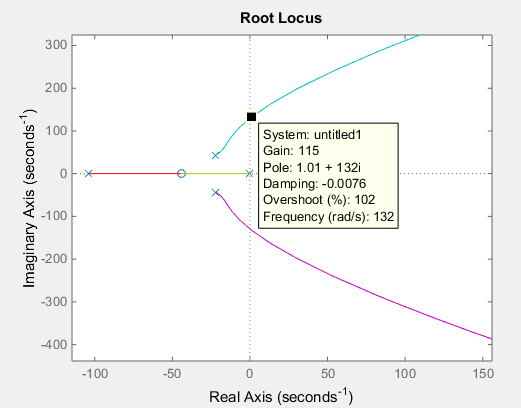
\includegraphics[scale=0.6]{Lugar-de-raices-con-integrador.png}
	\caption{Lugar de raíces con el integrador.}
	\label{fig:lugar-de-raices-con-integrador}
\end{figure}

\noindent En la figura \ref{fig:lugar-de-raices-con-integrador} se puede observar que, para que se mantenga la estabilidad del sistema, la ganancia del integrador ($K_{int}$) debe ser menor a 107. Teniendo esto en cuenta, en la figura \ref{fig:respuesta-al-escalon-con-k-1-M-30} se muestra la respuesta al escalón del sistema compensado con el integrador para una ganancia de $K_{int}=1$. Por otro lado, para obtener una salida positiva es necesario considerar el bloque F del diagrama \ref{fig:diag-externo_real_positiva_dig} como una ganancia unitaria negativa.


\begin{figure}[H]
	\centering
	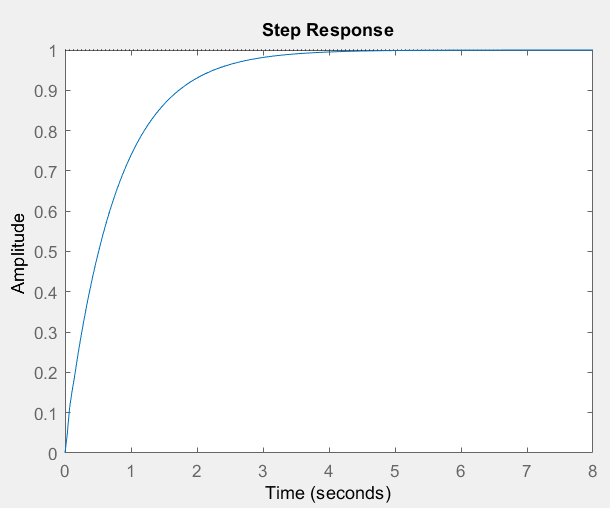
\includegraphics[scale=0.85]{Respuesta-al-escalon-con-k-1-M-30.png}
	\caption{Respuesta al escalón con integrador con $K_{int} =1$ y $M=30\:kg$.}
	\label{fig:respuesta-al-escalon-con-k-1-M-30}
\end{figure}


Al observar la figura \ref{fig:respuesta-al-escalon-con-k-1-M-30} es posible notar que la respuesta al escalón, si bien no posee oscilaciones, tiene un tiempo de establecimiento de  $2.94\:s$. Por lo tanto, para que el sistema presente mayor velocidad de respuesta, se decide aumentar el valor de ganancia hasta obtener una relación aceptable entre este tiempo y el sobrepico.

En la figura \ref{fig:respuesta-al-escalon-con-k-5-M-30}, se observa la respuesta al escalón para una ganancia del integrador de $K_{int}=5$ que resulta en un tiempo de establecimiento de $0.626\:s$ sin sobrepicos. Por lo tanto, se adopta este valor de ganancia para el diseño del integrador. Finalmente la transferencia del compensador externo queda:

\begin{equation} \label{eq_gexterno_dig}
	G_{ext}(w)=\frac{5}{w}	
\end{equation}

\colorbox{red}{creo que sería mas correcto poner la transferencia final del compensador en z --> Para mi no se si sirve de mucho en Z xq esto después hay que multiplicarlo por las transferencias(de la tlc interna) en W y pasar todo eso junto a Z} solamente las transferencias de los compensadores se pasan a z, no se multiplica todo junto

\begin{figure}[H]
	\centering
	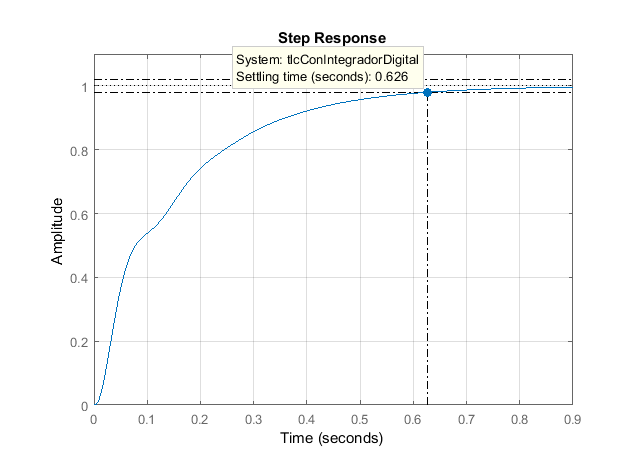
\includegraphics[scale=0.7]{Respuesta-al-escalon-con-k-5-M-30.png}
	\caption{Respuesta al escalón con integrador para $K_{int} =5$ y $M = 30\:kg$.}
	\label{fig:respuesta-al-escalon-con-k-5-M-30}
\end{figure}



%\begin{figure}[H]
%	\centering
%	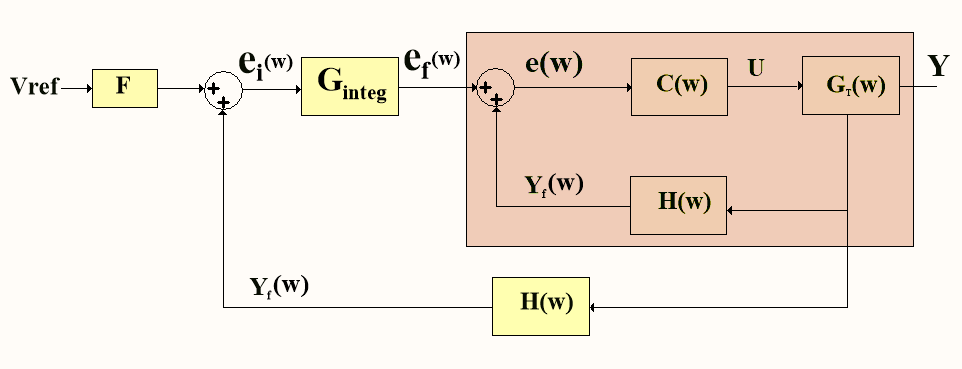
\includegraphics[scale=0.4]{Diagrama-del-sistema-completo.png}
%	\caption{Diagrama del sistema completo.}
%	\label{fig:diagrama-del-sistema-completo}
%\end{figure}



 La respuesta al escal\'{o}n cuando la masa es de $1\:kg$ se muestra en la figura \ref{fig:respuesta-al-escalon-con-k-5-M-1}. Allí se puede observar que el tiempo de establecimiento es de $0.752\:s$ y tampoco presenta sobrepicos.



\begin{figure}[H]
	\centering
	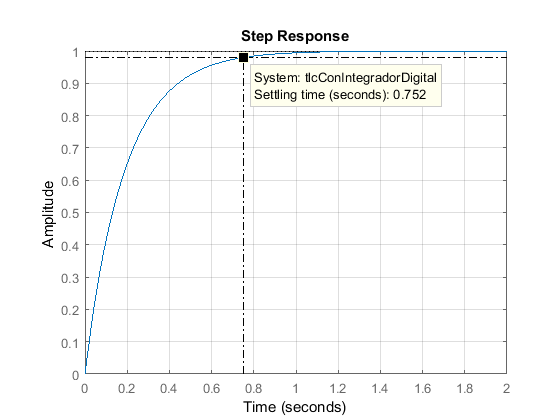
\includegraphics[scale=0.85]{Respuesta-al-escalon-con-k-5-M-1.png}
	\caption{Respuesta al escalón con integrador para $K_{int} =5$ y $M=1\:kg$.}
	\label{fig:respuesta-al-escalon-con-k-5-M-1}
\end{figure}

\subsection{Cálculo de ganancia de entrada}

Como se utiliza un controlador del tipo integrador, la señal a la salida del sumador ($Ve_{ext}$) será igual a cero en régimen permanente. Por lo tanto, como se desea que la salida $Y_g$ sea exactamente la misma que indica la referencia $Y_{ref}$, se debe cumplir la siguiente ecuación:

\begin{equation}
	Y_{ref}*F+Y_g=0
\end{equation}

Como $Y_{ref}=Y_g$, se obtiene $F=-1$.

\subsection{Transferencia de lazo cerrado}

Finalmente se puede expresar la función transferencia del lazo de control externo como:

\begin{equation}
	TLC_{externa}(w)=\frac{Y_g}{V_{y_{ref}}}=\frac{F*G_{ext}*TLC_{interna}}{1-G_{ext}*TLC_{interna}}
	%	\frac{-3.6301*}{den}
\end{equation}

%   0.00043659 (s+1.237e04) (s-1.238e04) (s-7143) (s+44.34)^2
%-----------------------------------------------------------
%(s+1196) (s+474.7) (s+99.01) (s+6.03) (s^2 + 39.87s + 2768)
Considerando que $F=-1$ y el caso de masa $M=30\:kg$ la transferencia de lazo cerrado queda:

\begin{equation*}
	\resizebox{.99\hsize}{!}
	{
		$
		TLC_{externa}(w)=\frac{4.37*10^{-4} (w+1.24*10^{4}) (w-1.24*10^{4}) (w-7143) (w+44.34)^2}{(w+1196) (w+474.7) (w+99.01) (w+6.03) (w^2 + 39.87w + 2768)}
		$
	}
\end{equation*}



\subsection{Cálculo de los coeficientes del controlador}


Se desea implementar el algoritmo de control en un microcontrolador. Esto significa obtener la señal de control $u[n]$ a partir de las entradas del sistema que son la referencia de posición ($Vref$) y la estimación ($Y[n]$). 

Para ello se obtienen las funciones transferencia de los compensadores diseñados en el dominio discreto (z). Para obtenerlas se aplica la transformada bilineal inversa a las transferencias del compensador por adelanto de fase $G_c(w)$ y al integrador $G_{ext}$. De esta forma, observando el diagrama de la figura \colorbox{red}{Ver diagrama} se plantea:

% 8.69e05 z^2 - 1.716e06 z + 8.477e05
%-----------------------------------
%z^2 - 1.551 z + 0.6018
%
%
%  8.69e05 - 1.716e06 z^-1 + 8.477e05 z^-2
%---------------------------------------
%1 - 1.551 z^-1 + 0.6018 z^-2

\begin{equation} \label{eq_coeficientes_interno} 
	G_c(z)=\ \ \frac{U(z)}{e(z)}=\frac{8.69*10^5- 1.72*10^6z^{-1} + 8.48*10^5z^{-2}}{1-1.551 z^{-1} + 0.6018 z^{-2}}\  
\end{equation} 
%0.0007 + 0.0007 z^-1
%--------------------
%1 - z^-1

\begin{equation} \label{eq_comp_externo_z} 
	G_{ext}(z)=\frac{e_f(z)}{e_i(z)}\ =\frac{0.0007(1+z^{-1})}{1-z^{-1}} 
\end{equation} 

Al aplicar la transformada inversa a las expresiones \ref{eq_coeficientes_interno} y \ref{eq_comp_externo_z} se obtiene:

\begin{equation} 
	\begin{aligned}\label{eq_U-coef}
		U[n]=&8.651*10^5e[n]-\ 1.709*10^6e[n-1]+\ 0.843*10^6e[n-2]+\\
		&+1.5514\ U[n-1]-\ 0.60171U[n-2]\\ 
	\end{aligned}
\end{equation}

\begin{equation} \label{eq_e-coef} 
	e_f[n]=0.0028*e_i[n]\ +\ {0.0028*e}_i[n-1]+e_f[n-1] 
\end{equation} 

Luego, para dejar el algoritmo de control en funci\'{o}n de las entradas del sistema, se debe reemplazar en las ecuaciones \ref{eq_U-coef} y \ref{eq_e-coef} las expresiones mencionadas en las ecuaciones \ref{GrindEQ__5_10_} y \ref{GrindEQ__5_11_}

\begin{equation} \label{GrindEQ__5_10_} 
	e[n]=e_f[n]+Y_f[n] 
\end{equation} 

\begin{equation} \label{GrindEQ__5_11_} 
	e_i[n]=F*Vref+Y_f[n] 
\end{equation} 


\section{Conexi\'{o}n entre el PCB y el microcontrolador}

 Se utiliza un conector tipo DB9 hembra como v\'{i}a de conexi\'{o}n para las distintas salidas y entradas digitales. Adem\'{a}s, en la placa se dispone de un led que se enciende cuando  se detecta una correcta conexi\'{o}n con el microcontrolador.
 
 \colorbox{red}{Ver de pasarlo a la sección del PCB y agregar tambien lo de capacitores de desacople, jumpers, leds, etc...}







